\documentclass[12pt, a4paper, oneside, final]{article}
\usepackage[margin = 1in, bottom = 1in]{geometry}

\usepackage[T2A]{fontenc}
\usepackage[utf8]{inputenc}
\usepackage[english, russian]{babel}
\usepackage{xcolor, ulem, soulutf8, soul, fancyhdr, amsmath, amssymb, amsthm, svg, wrapfig, csvsimple, float, caption, subcaption}
\usepackage[shortlabels]{enumitem}
\usepackage{titlesec, hyperref, multicol, listings}
\usepackage[most]{tcolorbox}
\usepackage[makeroom]{cancel}
\usepackage[most]{tcolorbox}
\usepackage{tocloft, longtable, skak, stmaryrd, color}
\usepackage[framemethod = tikz]{mdframed}

\definecolor{codegreen}{rgb}{0,0.6,0}
\definecolor{codegray}{rgb}{0.5,0.5,0.5}
\definecolor{codepurple}{rgb}{0.58,0,0.82}
\definecolor{backcolour}{rgb}{0.95,0.95,0.92}
\definecolor{blueish}{rgb}{0.96,0.96,1.0}
\definecolor{grayblueish}{rgb}{0.97,0.97,0.98}
\definecolor{transblue}{rgb}{0.9,0.9,0.97}
\definecolor{transred}{rgb}{0.97,0.9,0.9}
\definecolor{light-gray}{gray}{0.95}

\renewcommand{\figurename}{}
\addto\captionsrussian{\renewcommand{\figurename}{}}
\captionsetup[table]{labelformat = empty}

\hypersetup{
	colorlinks,
	citecolor = pink,
	filecolor = pink,
	linkcolor = pink,
	urlcolor = pink
}

\newtcblisting{mylisting}{
	listing only,
	breakable,
	colback = backcolour,
	enhanced jigsaw,
	sharp corners,
	boxrule = 0pt,
	frame hidden,
	listing options = {
		mathescape,
		commentstyle = \color{codegreen},
		keywordstyle = \color{magenta},
		numberstyle = \tiny\color{codegray},
		stringstyle = \color{codepurple},
		basicstyle = \ttfamily\footnotesize,
		breakatwhitespace = false,
		breaklines = true,
		captionpos = b,
		keepspaces = true,
		numbers = left,
		numbersep = 5pt,
		showspaces = false,
		showstringspaces = false,
		showtabs = false,
		tabsize = 4,
		inputencoding = utf8,
		language = python
	}
}

\binoppenalty = 10000
\relpenalty = 10000
\sloppy

\renewcommand*{\theenumi}{\thesection.\arabic{enumi}}
\renewcommand*{\theenumii}{\alph{enumii}}
\renewcommand*{\labelitemi}{\ensuremath{\triangleright}}

\everymath{\displaystyle}

\begin{document}
	\thispagestyle{empty}
	\vspace*{0.5em}
	\begin{center}
		{Национальный исследовательский университет ИТМО\\Факультет информационных технологий и программирования\\Прикладная математика и информатика}\\[5.0em]
		{\Huge \bfseries Методы оптимизации}\\[0.5em]
		{\large Отчет по лабораторной работе №2}\\[0.5em]
		\textcolor{gray}{\textlangle Собрано \today\textrangle}
	\end{center}
	\begingroup
	\def\hd{\begin{tabular}{ll}
			\textbf{Работу выполнили:} \\ Бактурин Савелий Филиппович M32331 \\ Вереня Андрей Тарасович M32331 \\ Сотников Максим Владимирович M32331 \vspace*{1em} \\
			\textbf{Преподаватель:} \\ TBA
		\end{tabular}
	}
	\vspace*{30em}
	\newlength{\hdwidth}
	\settowidth{\hdwidth}{\hd}
	\hfill\begin{minipage}{\hdwidth}\hd\end{minipage}
	\endgroup
	\newpage
	\section*{Стохастический градиентный спуск}
	\subsection*{Исследование с разными размерами батча}
	Реализуйте стохастический градиентный спуск для решения линейной регрессии.
	Исследуйте сходимость с разным размером батча ($1$~-- SGD, $2$, $\dots$, $n - 1$~-- Minibatch GD, $n$~-- GD из предыдущей работы).
	\subsubsection*{Стохастический градиентный спуск}
	\textit{Стохастический градиентный спуск}~--- модификация к основному методу итерационного поиска минимума через антиградиент дифференцируемой функции в рассматриваемой плоскости $\mathbb{R}^{n}$.
	Идея: пусть есть множество $M$~-- какой-то полный набор данных вычисленных оценок при спуске к минимуму, тогда в рассматриваемой версии мы будем брать случайное значение из выбранного $M' \subset M$.
	Как правило, такой подход преуменьшает вычислительные ресурсы, в особенности, следует помнить, что $\mathtt{float}$ считается крайне медленно, и ускоряет итерацию по количествам эпохам, но при этом мы теряем точность сходимости.

	Пусть $x_{i} = \{x_i^0, x_i^1, ~ \ldots, x_i^{n - 1}\}$~-- координата в $\mathbb{R}^{n}$ и задана функция $f(x_i) : \mathbb{R}^{n} \to \mathbb{R}$.
	Мы хотим нашу задачу свести к исследованию на некоторых специальных образцах заданной функции, для каждой точки из которых мы будем минимизировать ошибку для дальнейшего нахождения приближенного минимума рассматриваемой функции $f(x_i)$.
	Мы хотим найти линейную регрессию, представляющая из себя полином $1$-ой степени от $n$ переменных.
	Для начала мы найдем функцию ошибки $S$ по следующей формуле:
	\[
		S(f) = (X'^{\mathrm{T}} \times X')^{-1} \times X'^{\mathrm{T}} \times Y \times \vec{x},
	\] где $Y$~-- матрица значений при множестве $X$ (определение), $X'$~-- это матрица $X$, но в $1$-ой колонке забитый единицами.
	По другому мы можем записать данную формулу следующим образом:
	\[
		S(f) = \sum\limits_{i = 1}^{N}{\left(y_{i} - x_{i} \cdot w_{i}\right)^{2}},
	\] где $y_{i} \in D(f(x_{i}))$ (образ функции), $w_{i} \in W$~-- сгенерированные веса, коэффициенты при линейной функции.

	Рассмотрим идею алгоритма.
	При итерации, пока мы не превысили максимальное количество шагов или не сведем нашу функцию потери до некоторого $\varepsilon$, мы будем обобщать экспериментальные данные в виде случайных точек в некоторую многомерную линию.
	На каждом шаге мы будем изменять функцию потерь от измененной $w$.

	Напишем идейный псевдокод.
	Скажем, что $x_{i} = \{x^{0}_{i}, ~ x^{1}_{i}, ~ \ldots, x^{n - 1}_{i}\}$~-- координата в $n$-мерном пространстве $\mathbb{R}^{n}$, $y_{i} = \{y^{0}_{i}, ~ y^{1}_{i}, ~ \ldots, y^{n - 1}_{i}\}$~-- образ функции $f(x_{i})$.
	\begin{mylisting}
function $\mathtt{S}(x, y, w)$:
	return $\sum\limits_{i = 1}^{N}{(y_{i} - x_{i} \cdot w_{i})^{2}}$

function $\mathtt{stochastic\_descent}(x, y)$:
	$w \gets$ [$w_{i} \in \mathbb{R}$] * n
	$\mathtt{prev} \gets INIT$, $\text{предыдущее значение функции потери}$
	$\mathtt{next} \gets S(x, y, w)$, $\text{текущее значение функции потери}$
	$\alpha \gets$ const
	while $|\mathtt{prev} - \mathtt{next}| > \varepsilon$:
		$\mathtt{prev} \gets \mathtt{next}$
		$i \gets x \in [0, ~ |Y|]$
		$T \gets$ [0] * n
		$\forall j \in |w|$ do
			$T_{j} \gets (y_{i} - x_{i} \times w) \cdot x_{i}^{j}$
		$w \gets w + \alpha \cdot T$
		$\mathtt{next} \gets S(x, y, w)$
	return $w$
	\end{mylisting}
	\paragraph{Пример с SGD, Minibatch, GD.}
	Для понимания контекста, давайте увидим разницу между рассматриваемым градиентным спуском, Minibatch и общим, с которым мы уже давно знакомы. Возьмем в качестве функции $f(x, y) = x^{2} + y^{2}$, тогда его градиентом будет $\dfrac{\partial{f}}{\partial{\vec{x}}} = 2x + 2y$, также для GD мы выставим следующие параметры:
	\begin{itemize}
		\item $\texttt{learning\_rate} = 0.1$
		\item $\varepsilon = 0.00001$
		\item $\texttt{max\_epoch} = 1000$~-- одно из условий остановки спуска, вторым~-- проверка, что мы сошлись.
	\end{itemize}
	Запустим и посмотрим на график всех трех джентльменов.
	\begin{figure}[H]
		\centering
		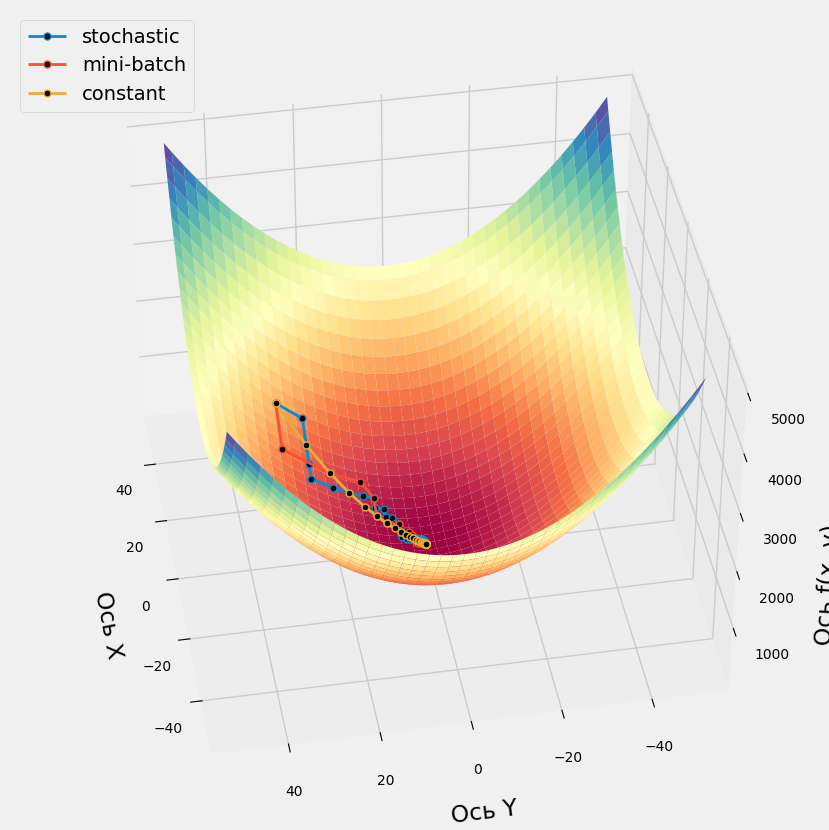
\includegraphics[scale = 0.5]{Image/T1_3d_FUNCTIONS.png}
		\caption*{SGD vs. Minibatch vs. GD}
	\end{figure}
	Полученные данные, после прохода алгоритмов, выглядят так:
	\begin{itemize}
		\item Для стохастического нашлась $f(0.002658, 0.00836) \approx 0.000008$.
		\item Для Minibatch~-- $f(0.002658, 0.000219) \approx 0.000007$.
		\item Для градиентного спуска (constant)~-- $f(0.001701, 0.002042) \approx 0.000007$.
	\end{itemize}
 	Точками отмечены шаги алгоритмов. Заметим, что в отличие GD, стохастический спуск уже с первого шага начинает идти не туда и, как можно приглядеться в минимуме функции, \textcolor{blue}{синяя} полоса пробирается то левее, то правее GD небольшими шагами. Minibatch также начинает свое \textcolor{red}{движение} не совсем по траектории GD, но в отличие от своего предшественника, быстрее начинает сходится к настоящей траектории.
	\subsubsection*{Minibatch градиентный спуск}
	Модификация \textit{Minibatch} обобщает вариант стохастического градиентного спуска, тем, что во время итерации мы будем брать не одну случайную точку из посчитанных на предыдущем шаге и изменять функцию потери как бы относительно её, а теперь возьмем выборку $M' \subset M$, причем, обязательно, чтобы $|M'| > 1$ и $|M'| < |M|$.

	Тогда псевдокод от предыдущего рассмотренного варианта почти ничем не отличается.
	Скажем также, что $x_{i} = \{x^{0}_{i}, ~ x^{1}_{i}, ~ \ldots, x^{n - 1}_{i}\}$~-- координата в $n$-мерном пространстве $\mathbb{R}^{n}$, $y_{i} = \{y^{0}_{i}, ~ y^{1}_{i}, ~ \ldots, y^{n - 1}_{i}\}$~-- образ функции $f(x_{i})$; значение $m$~-- выступает в роли мощности подмножества $M'$.
	\begin{mylisting}
function $\mathtt{S}(x, y, w)$:
	return $\sum\limits_{i = 1}^{N}{(y_{i} - x_{i} \cdot w_{i})^{2}}$
	
function $\mathtt{stochastic\_descent}(x, y, m)$:
	$w \gets$ [$w_{i} \in \mathbb{R}$] * n
	$\mathtt{prev} \gets INIT$, $\text{предыдущее значение функции потери}$
	$\mathtt{next} \gets S(x, y, w)$, $\text{текущее значение функции потери}$
	$\alpha \gets$ const
	while $|\mathtt{prev} - \mathtt{next}| > \varepsilon$:
		$\mathtt{prev} \gets \mathtt{next}$
		$\forall i \in [0, m]$ do
			$T \gets$ [0] * n
			$\forall j \in |w|$ do
				$T_{j} \gets (y_{i} - x_{i} \times w) \cdot x_{i}^{j}$
			$w \gets w + \alpha \cdot T$
		$\mathtt{next} \gets S(x, y, w)$
	return $w$
	\end{mylisting}
	\subsubsection*{Градиентный спуск}
	Наконец, самый общий случай и являющийся самым быстроходным среди двух рассмотренных ранее, благодаря тому, что мы учитываем все точки $M' \equiv M$.
	Данный метод работает крайне медленно, но является одним из самых быстрых в сходимости к приближенной точке минимума.

	Пусть $m$~-- есть мощность множества $M$, тогда идейным псевдокодом-решением задачи будет являться тот же код, что и для предыдущего варианта, то есть
	\begin{mylisting}
function $\mathtt{S}(x, y, w)$:
	return $\sum\limits_{i = 1}^{N}{(y_{i} - x_{i} \cdot w_{i})^{2}}$
	
function $\mathtt{stochastic\_descent}(x, y, m)$:
	$w \gets$ [$w_{i} \in \mathbb{R}$] * n
	$\mathtt{prev} \gets INIT$, $\text{предыдущее значение функции потери}$
	$\mathtt{next} \gets S(x, y, w)$, $\text{текущее значение функции потери}$
	$\alpha \gets$ const
	while $|\mathtt{prev} - \mathtt{next}| > \varepsilon$:
		$\mathtt{prev} \gets \mathtt{next}$
		$\forall i \in [0, m]$ do
			$T \gets$ [0] * n
			$\forall j \in |w|$ do
				$T_{j} \gets (y_{i} - x_{i} \times w) \cdot x_{i}^{j}$
		$w \gets w + \alpha \cdot T$
	$\mathtt{next} \gets S(x, y, w)$
	return $w$
	\end{mylisting}
	\paragraph{Исследование Stohastic vs. Minibatch vs. GD.}
	В качестве рассматриваемого пространства $\mathbb{R}^{2}$, где $2 = \texttt{количество\_весов} + \texttt{<<результирующий\_вес>>}$, для $X \subset \mathbb{N}$ мы возьмем множество $\{x\}_{i = 1}^{n}$, где $n \gets 500$ и $x_{i} < x_{i + 1}$.
	Возьмем в качестве генерируемой прямой в пространстве одного из наиболее известного представителя фауны функции потерь, называемый \textit{MSE}.
	Построим график исследования $\texttt{эпохи}(\texttt{batch\_size})$, где под \textit{эпохами} мы определяем количество шагов до сходимости к значению функции потерь на реальных данных с $\pm$ точности, порядка, стремящихся к нулю.
	Построим график.
	\begin{figure}[H]
		\centering
		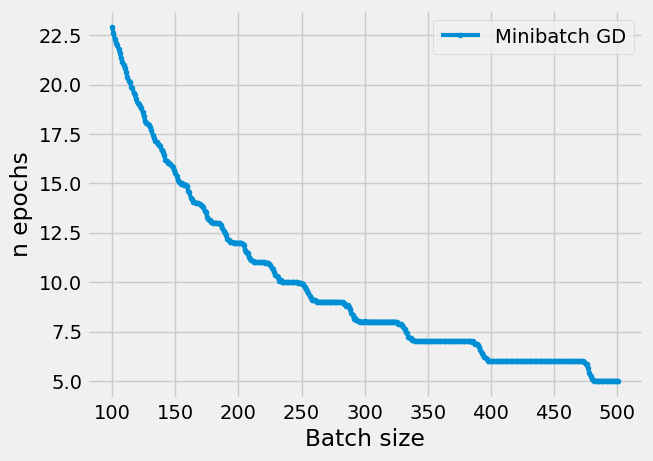
\includegraphics[scale = 0.55]{Image/T1_ECHOES_BATCHSIEZ.png}
		\caption*{SGD vs. Minibatch vs. GD}
	\end{figure}
	Итак проанализируем.
	Мы уже знаем, что стохастический градиентный спуск и Minibatch в внезапный момент начинают идти куда-либо, только не по направлению анти-градиента.
	Замечаем также, особенность в Minibatch: существуют некоторые $n_{i} : \exists n'_{i} : n_{i} < n'_{i}, ~ \forall n'' \in [n_{i}, n'_{i}] ~ \texttt{epoechs}(n'') = \texttt{const}$.
	Другими словами: существуют некоторые периоды $\pi_{i}$, при которых количество шагов до сходимости не меняются.
	При этом, замечаем $\forall i$ верно, что $|\pi_{i}| < |\pi_{i + 1}|$, что, вероятнее всего, связано с размером батча и генерируемых весов точек, заданных уже имплементацией лабораторной работы.
	Почти полная таблица того, как именно изменяются количества эпох:
	\begin{table}[H]
		\centering
		\begin{tabular}{|c|c|}
			Batch size & $\text{Кол-во эпох}_{\times 10^2}$ \\ \hline
			100 & 2229 \\
			101 & 2202 \\
			102 & 2186 \\
			103 & 2169 \\
			104 & 2136 \\
			105 & 2121 \\
			106 & 2099 \\
			107 & 2085 \\
			$\vdots$ & $\vdots$ \\
			208 & 1102 \\
			209 & 1102 \\
			210 & 1100 \\
			211 & 1100 \\
			212 & 1100 \\
			213 & 1100 \\
			214 & 1099 \\
			215 & 1099 \\
			216 & 1097 \\
			$\vdots$ & $\vdots$ \\
			468 & 512 \\
			469 & 501 \\
			470 & 500 \\
			471 & 501 \\
			472 & 500 \\
			473 & 500 \\
			$\vdots$ & $\vdots$ \\
			494 & 500 \\
			495 & 500 \\
			496 & 500 \\
			497 & 500 \\
			498 & 500 \\
			499 & 500 \\
			500 & 500
		\end{tabular}
	\end{table}
	\subsection*{Learning rate scheduling}
	Задачей мы поставим подбор функции изменения шага, чтобы улучшить сходимость из предыдущего пункта.
	Тогда, мы использовали самый простой способ~-- \textit{константный}, однако у него есть недостаток: иногда шаг в $\mathtt{const\_learning\_rate}$ может <<перепрыгнуть>> через минимум и/или начать <<прыгать>> через него бесконечно много раз, в таком случае мы хотим, чтобы шаг был уменьшен.
	Другой случай: когда такой шаг может привести к долгому ожиданию, пока алгоритм не дойдет до минимума.
	Вот тут и возникает задача подбора такой функции изменения шага, чтобы алгоритм за какое-то конечное $k$ эпох добрался до минимума быстрее. 
	В качестве такой мы возьмем \textit{экспоненциальную функцию}.
	Экспоненциальная функция, в общем случае, для изменения сходимости выглядит так:
	\[
		\mathtt{learning\_rate} = \mathtt{start\_learning\_rate} \cdot e^{-k \cdot \mathtt{epoch}},
	\] где $\mathtt{learning\_rate}$~-- текущий размер шага, $\mathtt{start\_learning\_rate}$~-- стартовая длина, $k$~-- некий параметр, который может зависеть от размера выбранного батча, и, наконец, $\mathtt{epoch}$~-- текущий номер эпохи.
	\paragraph{Пример с $f(x) = 2x + 0$.}
	Для линейной регрессии рассмотрим в качестве функции $f(x) = 2x + 0$, где $a = 2$ и $b = 0$.
	Сравним разницу между константным и экспоненциальной функциями потерь, где в качестве значения $k \gets 0.05$ и \texttt{epoch} будем считать следующим образом: $(\texttt{current\_epoch} + 10)$.
	Рассмотрим следующую зависимость: \texttt{значение\_функции\_потерь(количество\_эпох)}.
	\begin{figure}[H]
		\centering
		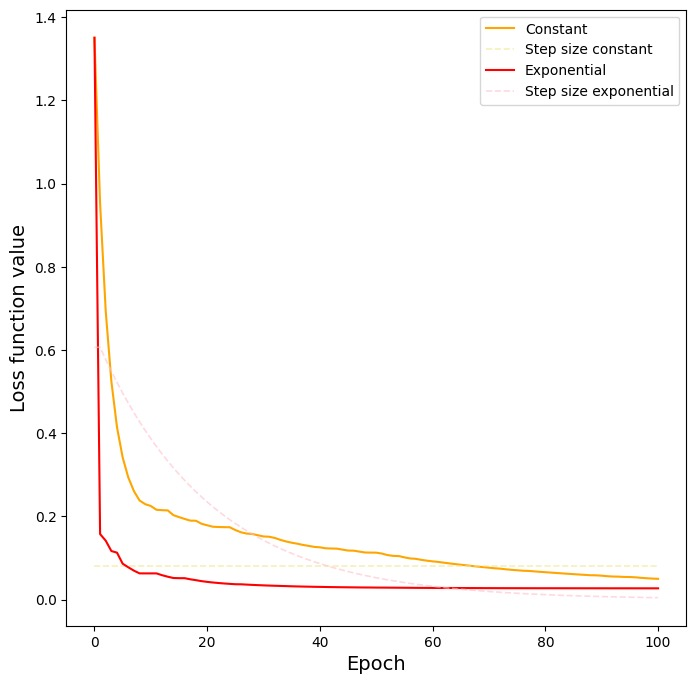
\includegraphics[scale = 0.68]{Image/T1_SGD_constantLR_expLR.jpeg}
		\caption*{Constant lr vs. Exponential lr}
	\end{figure}
	Как можно заметить, константный метод по очевидным причинам хуже сходится (параллельная линия оси ординат), экспоненциальная же понемногу (на самом деле, по многу) начинает быстрее сходится из-за присутствия <<минуса>> в степени и, соответственно, меньшим lr.
	\paragraph{SGD и разные функции потерь.}
	Как и в предыдущей задаче, мы рассмотрим линейную регрессию, но в качестве исследования мы возьмем других не менее известных представителей функций потерь:
	\begin{align*}
		\text{MAE} &= \dfrac{\sum\limits_{i = 1}^{n}{|y_{i} - x_{i}|}}{n} \\
		L_{\delta}(a) &=
		\begin{cases}
			\dfrac{1}{2} \cdot a^{2}, ~ |a| \leqslant \delta, \\
			\delta \cdot \left(|a| - \dfrac{1}{2} \cdot \delta\right)
		\end{cases}, ~ \text{где} ~ a = y - f(x) \\
		\text{logcosh} &= \log{\left(\dfrac{e^{y_{\text{pred}} - y_{\text{real}}} + e^{-y_{\text{pred}} + y_{\text{real}}}}{2}\right)} \\
		\text{quantile} &=
		\begin{cases}
			\alpha \cdot (y_{\text{real} - y_{\text{pred}}}), ~ y_{\text{real} - y_{\text{pred}}} \geqslant 0 \\
			(\alpha - 1) \cdot (y_{\text{real} - y_{\text{pred}}})
		\end{cases}
	\end{align*}
	 На сей раз, мы рассмотрим линейную функцию $f(x) = 2x - 1$.
	 Для каждого из функций потерь построим pred-функцию и сравним их эффективность в плане восстановления до исходной прямой.
	\begin{figure}[H]
		\centering
		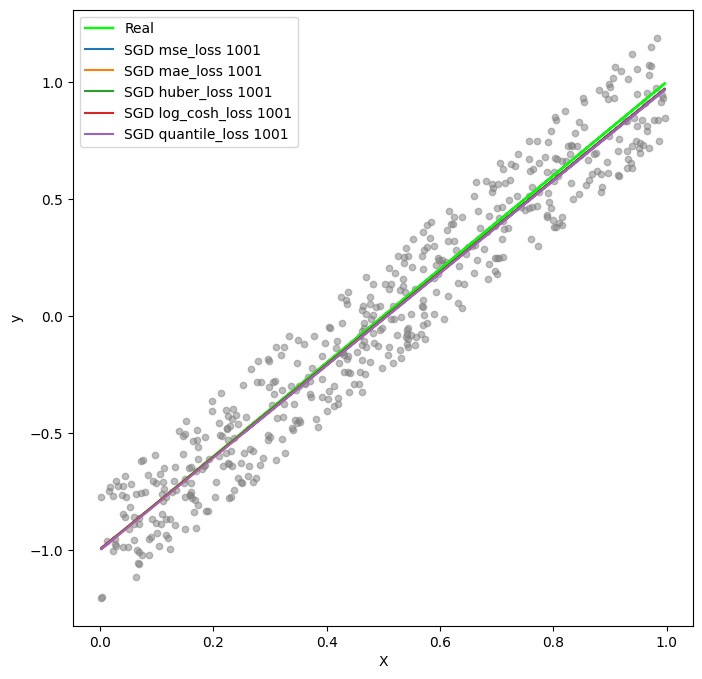
\includegraphics[scale = 0.6]{Image/T1_SGD_with_LOSS_FUNCTIONS.jpeg}
		\caption*{Real vs. mae vs. mse vs. huber vs. logcosh vs. quantile}
	\end{figure}
	Для нее мы задали следующие настройки алгоритма:
	\begin{itemize}
		\item Количество генерируемых весов~-- $5000$.
		\item $\varepsilon \gets 0.0085$
		\item $\texttt{learning\_rate} \gets 0.1$
		\item Максимальное число до сходимости~-- $1000$.
	\end{itemize}
	Заметим, что почти все методы отработали почти \textcolor{green}{одинаково} и совпали с настоящей прямой.
	Полные результаты коэффициентов уравнений прямой такие:
	\begin{align*}
		\text{MSE} &\to y = 2.002 \cdot x - 1.000 \\
		\text{MAE} &\to y = 2.005 \cdot x - 1.002 \\
		\text{HUBER} &\to y = 1.999 \cdot x - 0.998 \\
		\text{LOGCOSH} &\to y = 1.999 \cdot x - 0.998 \\
		\text{QUANTILE} &\to y = 2.006 \cdot x - 1.002
	\end{align*}
	\paragraph{Minibatch и разные функции потерь.}
	Как и в прошлом примере, мы возьмем функцию $f(x) = 2x - 1$ и те же разные местные представители фауны из предыдущего пункта.
	Однако, теперь мы возьмем Minibatch GD и составим график на сей раз $\texttt{значение\_функции\_потери}(\texttt{эпохи})$.
	Настройки для алгоритма такие же, как и в прошлом пункте.
	Запустим и проанализируем:
	\begin{figure}[H]
		\centering
		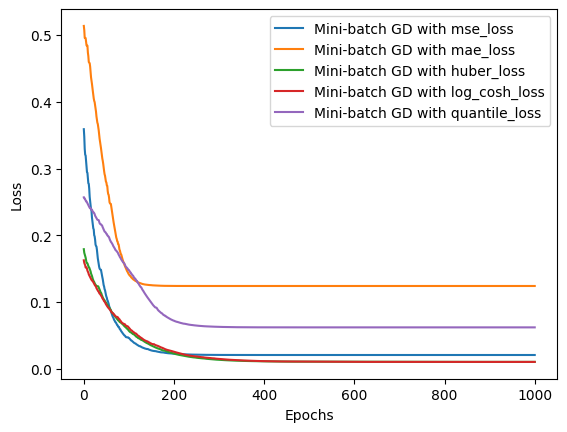
\includegraphics[scale = 0.78]{Image/T1_MINIBATCH_with_LOSS_FUNCTIONS.png}
		\caption*{Minibatch vs. loss functions}
	\end{figure}
	И мы получаем две категории победы у разных функций:
	\begin{itemize}
		\item По быстроте (то есть, по количеству эпох) сходимости (то есть, когда мы получаем параллельную прямую над осью ординат)~-- $\text{MAE}$, при этом эта функция проигрывает следующей категории.
		\item По аргументу (то есть, по значению функции потерь)~-- получаем вровень идущих $L_{\delta}(a)$ и $\text{logcosh}$, приближающееся к нулю.
	\end{itemize}
	Полные результаты значений функций потерь:
	\begin{align*}
		\text{MSE} &\to
		\begin{cases}
			\text{REAL} = 0.02061322422787911 \\
			\text{MSE} = 0.020611644279003895 \\
			\text{DIFF} = -1.579948875216064e-06
		\end{cases} \\
		\text{MAE} &\to
		\begin{cases}
			\text{REAL} = 0.12404634033734865 \\
			\text{MAE} = 0.12403644707794269 \\
			\text{DIFF} = -9.89325940596586e-06
		\end{cases} \\
		\text{HUBER} &\to
		\begin{cases}
			\text{REAL} = 0.010306612113939555 \\
			\text{HUBER} = 0.010306151224572697 \\
			\text{DIFF} = -4.6088936685867443e-07
		\end{cases} \\
		\text{LOGCOSH} &\to
		\begin{cases}
			\text{REAL} = 0.010242649302131148 \\
			\text{LOGCOSH} = 0.01024226833627978 \\
			\text{DIFF} = -3.809658513671127e-07
		\end{cases} \\
		\text{QUANTILE} &\to
		\begin{cases}
			\text{REAL} = 0.06202317016867433 \\
			\text{QUANTILE} = 0.062018214022529945 \\
			\text{DIFF} = -4.956146144381723e-06
		\end{cases}
	\end{align*}
	\subsection*{Исследование различных модификаций}
	Исследуйте модификации градиентного спуска (Nesterov, Momentum, AdaGrad, RMSProp, Adam).
	\subsubsection*{Momentum}
	Пусть нам дана функция $f(x_{i})$, где $x_{i} = \{x_{i}^{1}, ~ x_{i}^{2}, ~ \ldots, ~ x_{i}^{n}\}$~-- координата точки $x_{i}$ в $n$-мерном пространстве~-- и пусть у данной $f$ есть множество локальных точек минимума, образующийся <<впадиной>> функции, и <<горы>>~-- максимумов.
	Рассмотрим некоторый \textit{объект} $\mathfrak{O}$, который обладает свойством <<скольжения>> по поверхности нашей функции $f$, определяемый следующим образом:
	\begin{enumerate}[a)]
		\item если он <<сходит>> с горы, то он не останавливается при <<схождении>> с локального максимума;
		\item если он <<перескакивает>> локальный минимум, то он либо остановится на идеально гладкой части поверхности функции $f$, либо он <<сойдет>> к локальному минимуму.
	\end{enumerate}
	Идея модификации градиентного спуска \textit{Momentum} в создании алгоритма, обладающий свойством $\mathfrak{O}$ в имении свойства импульса.

	Рассмотрим последовательность $\{u_{i}\}$, которую мы назовем <<скоростью>>, скажем, что $\{g_{i}\} \equiv \{-\nabla{f(x_{i})}\}$, тогда определим скорость следующим образом:
	\[
		v_{i + 1} = \lambda \cdot v_{i} + (1 - \lambda) \cdot g_{i}, ~ \lambda \in (0, 1)
	\] и зададим изменение на $i + 1$-ой итерации наших весов точек:
	\[
		w_{i + 1} = w_{i} - \alpha \cdot v_{i + 1}, ~ \alpha = \mathtt{const}
	\]
	Здесь и во всех ниже рассматриваемых модификациях стохастического градиентного спуска мы будем рассматривать в качестве функции потерь функцию \textit{MSE}.
	Настроим наше исследование и запустим с следующими параметрами:
	\begin{itemize}
		\item Максимальное количество эпох~-- $4000$.
		\item Начальным \texttt{learning\_rate}~-- $0.001$.
		\item Количество генерируемых точек~-- $500$.
	\end{itemize}
	Важное замечание: здесь и далее мы будем ограничивать по количество шагов алгоритма.
	Если оно превысило число генерируемых точек, то алгоритм останавливается и передается новое значение батча.
	Рассмотрим же график для \textit{Momentum}.
	\begin{figure}[H]
		\centering
		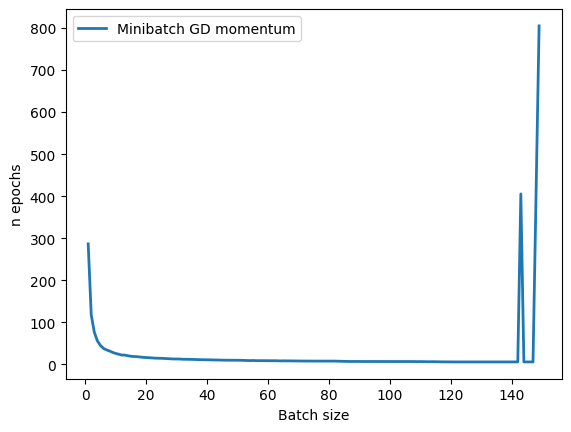
\includegraphics[scale = 0.78]{Image/T3_MOMENTUM_GENERAL.png}
		\caption*{Momentum in general}
	\end{figure}
	Заметим, что изначально, как и ожидается, алгоритм быстро сходится при больших числах размерах батча.
	Однако, в какой-то момент, число шагов резко возрастает и, можно заметить, что в среднем зависимость будет перепадать на сам батч, чем на веса.
	Это происходит из-за многих проблем: одна из которых заключается в том, что наши шаги становятся слишком маленькие настолько, что максимальное число эпох не покрывает в пределе.

	Более детальное изображение Momentum при первых десяти batch размерах:
	\begin{figure}[H]
		\centering
		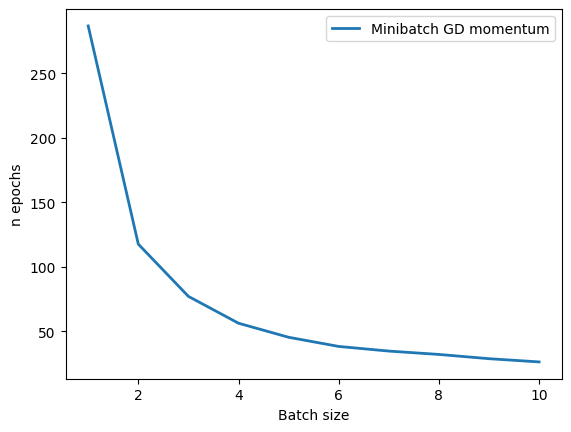
\includegraphics[scale = 0.78]{Image/T3_MOMENTUM_1_10.png}
		\caption*{Momentum in $[1, 10]$}
	\end{figure}
	\subsubsection*{Nesterov}
	Модификация \textit{Nesterov} по своей сути почти ничем не отличается ранее рассмотренного Momentum: единственное, что отделяет братьев по крови, так это то, что Nesterov считает градиент не в текущей точке, на которой мы стоим, а той, куда мы бы могли пойти, следуя импульсу.
	Тогда, наши основные формулы немного меняются, для скорости:
	\[
		v_{i + 1} = \lambda \cdot v_{i} + (1 - \lambda) \cdot g(w_{i} - \alpha \cdot \lambda \cdot v_{i}), ~ \alpha = \mathtt{const}
	\]
	И для весов:
	\[
		w_{i + 1} = w_{i} - \alpha \cdot v_{i + 1}
	\]
	Для исследования алгоритма мы выставим ровно те же настройки, что были у Momentum.
	Рассмотрим же график для Nesterov.
	\begin{figure}[H]
		\centering
		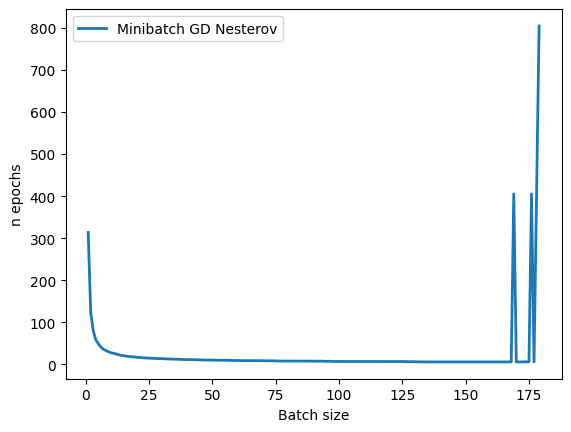
\includegraphics[scale = 0.78]{Image/T3_NESTEROV_GENERAL.png}
		\caption*{Nesterov in general}
	\end{figure}
	Замечаем, что количество шагов не сильно (иначе говоря, не хуже), чем в предыдущем рассмотренном пациенте.
	Однако, проблема с шагами остается, чему является подтверждение на последних итерациях batch размеров.

	Более детальное изображение Nesterov при первых десяти batch размерах:
	\begin{figure}[H]
		\centering
		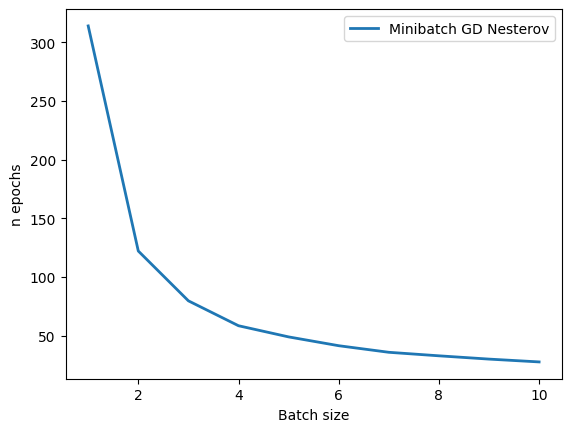
\includegraphics[scale = 0.78]{Image/T3_NESTEROV_1_10.png}
		\caption*{Nesterov in $[1, 10]$}
	\end{figure}
	\subsubsection*{AdaGrad}
	Рассмотрим некий $\mathtt{start\_learning\_rate}$ и стандартный метод стохастического спуска.
	Как мы уже видели, одним из недостатков такого метода является появления слишком больших или, наоборот, маленьких компонент относительно друг друга.
	Для исправления мы введём матрицу $\Omega$, которую определим следующим образом:
	\[
		\Omega = \sum\limits_{j = 1}^{i}{g_{j} \times g_{j}^{\mathrm{T}}},
	\] где $g_{j}$~-- $\nabla{f(x_{j})}$.
	Теперь рассмотрим основную формулу и поделим часть, где идет <<шаг>> алгоритма, на $\Omega_{i, i}$:
	\[
		w_{i + 1} = w_{i} - \dfrac{\alpha \cdot g_{j}}{\sqrt{\Omega_{i, i}}}
	\]
	Теперь же, там, где мы потенциально делаем большие шаги, мы делим на большое $\Omega_{i, i}$ и таким образом уменьшаем количество больших скачков.
	Тут мы получаем глобальную проблема в виде потенциально слишком высокой скорости уменьшения шага.

	Настроим наше исследование и запустим с следующими параметрами:
	\begin{itemize}
		\item Максимальное количество эпох~-- $4000$.
		\item Начальным \texttt{learning\_rate}~-- $0.1$.
		\item Количество генерируемых точек~-- $500$.
		\item В качестве константы положим $\alpha = 1e-5$.
	\end{itemize}
	Рассмотрим же график для AdaGrad.
	\begin{figure}[H]
		\centering
		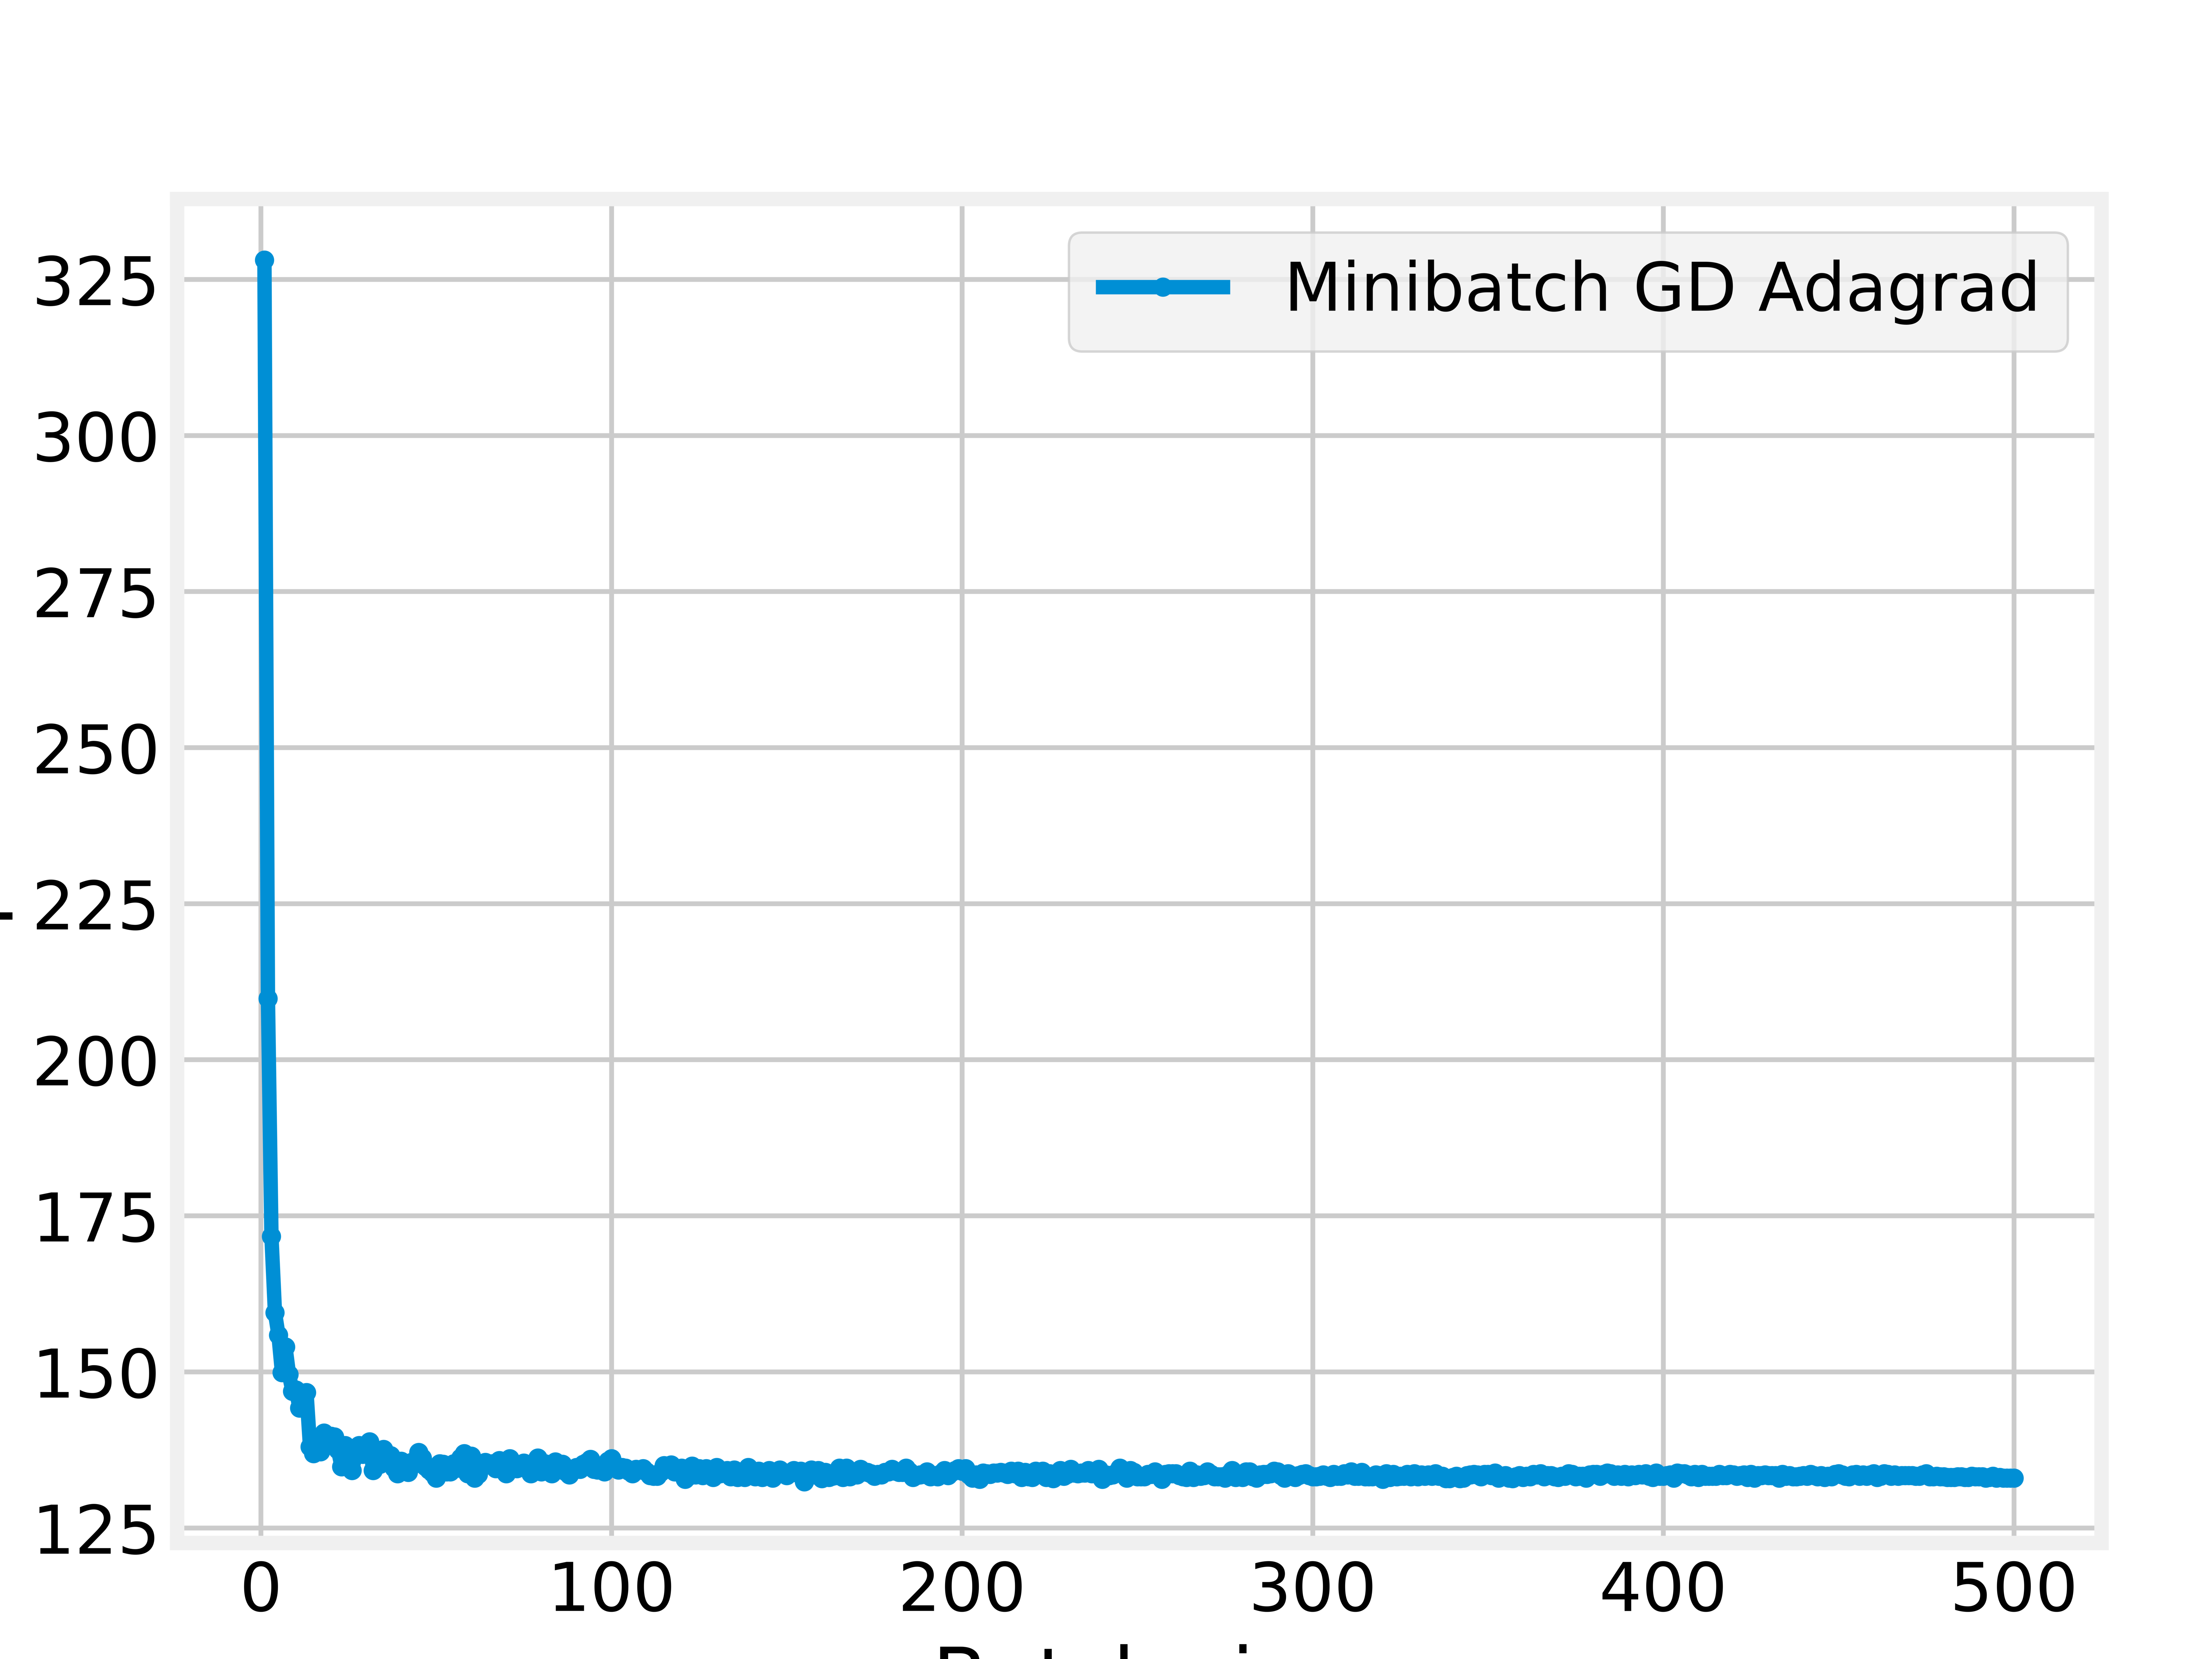
\includegraphics[scale = 0.9]{Image/T3_ADAGRAD_GENERAL.png}
		\caption*{AdaGrad in general}
	\end{figure}
	Количество шагов, из-за все ещё нерешенной глобальной проблемы, стало в среднем немного хуже, чем в предыдущих модификациях, однако здесь мы не видим каких-либо резких возвышений и перепадов.
	Также заметим, что график функции выглядит не как линия, а как некий <<шум>>, резко перебегающей функцией то вверх, то вниз.
	\subsubsection*{RMSProp}
	Модификация \textit{RMSProp} решает возникшую проблему с AdaGrad, в качестве решения было предложено усреднять значения.
	Пусть $(g_{i})^{2}$~-- покомпонентное возведение в квадрат, $\eth$~-- некое число порядка $[10^{-10}, ~ 10^{-7}]$, дабы по формуле не было деления на ноль.
	Тогда, в качестве скорости возьмем:
	\[
		s_{i + 1} = \lambda \cdot s_{i} + (1 - \lambda) \cdot (g_{i})^{2}, ~ \lambda \in (0, 1)
	\]
	Наконец, изменение весов:
	\[
		w_{i + 1} = w_{i} - \alpha \cdot \dfrac{g_{i}}{\sqrt{s_{i + 1} + \eth}}, ~ \alpha = \mathtt{const}
	\]
	Для исследования алгоритма мы выставим ровно те же настройки, что были у AdaGrad.
	Рассмотрим же график для RMSProp.
	\begin{figure}[H]
		\centering
		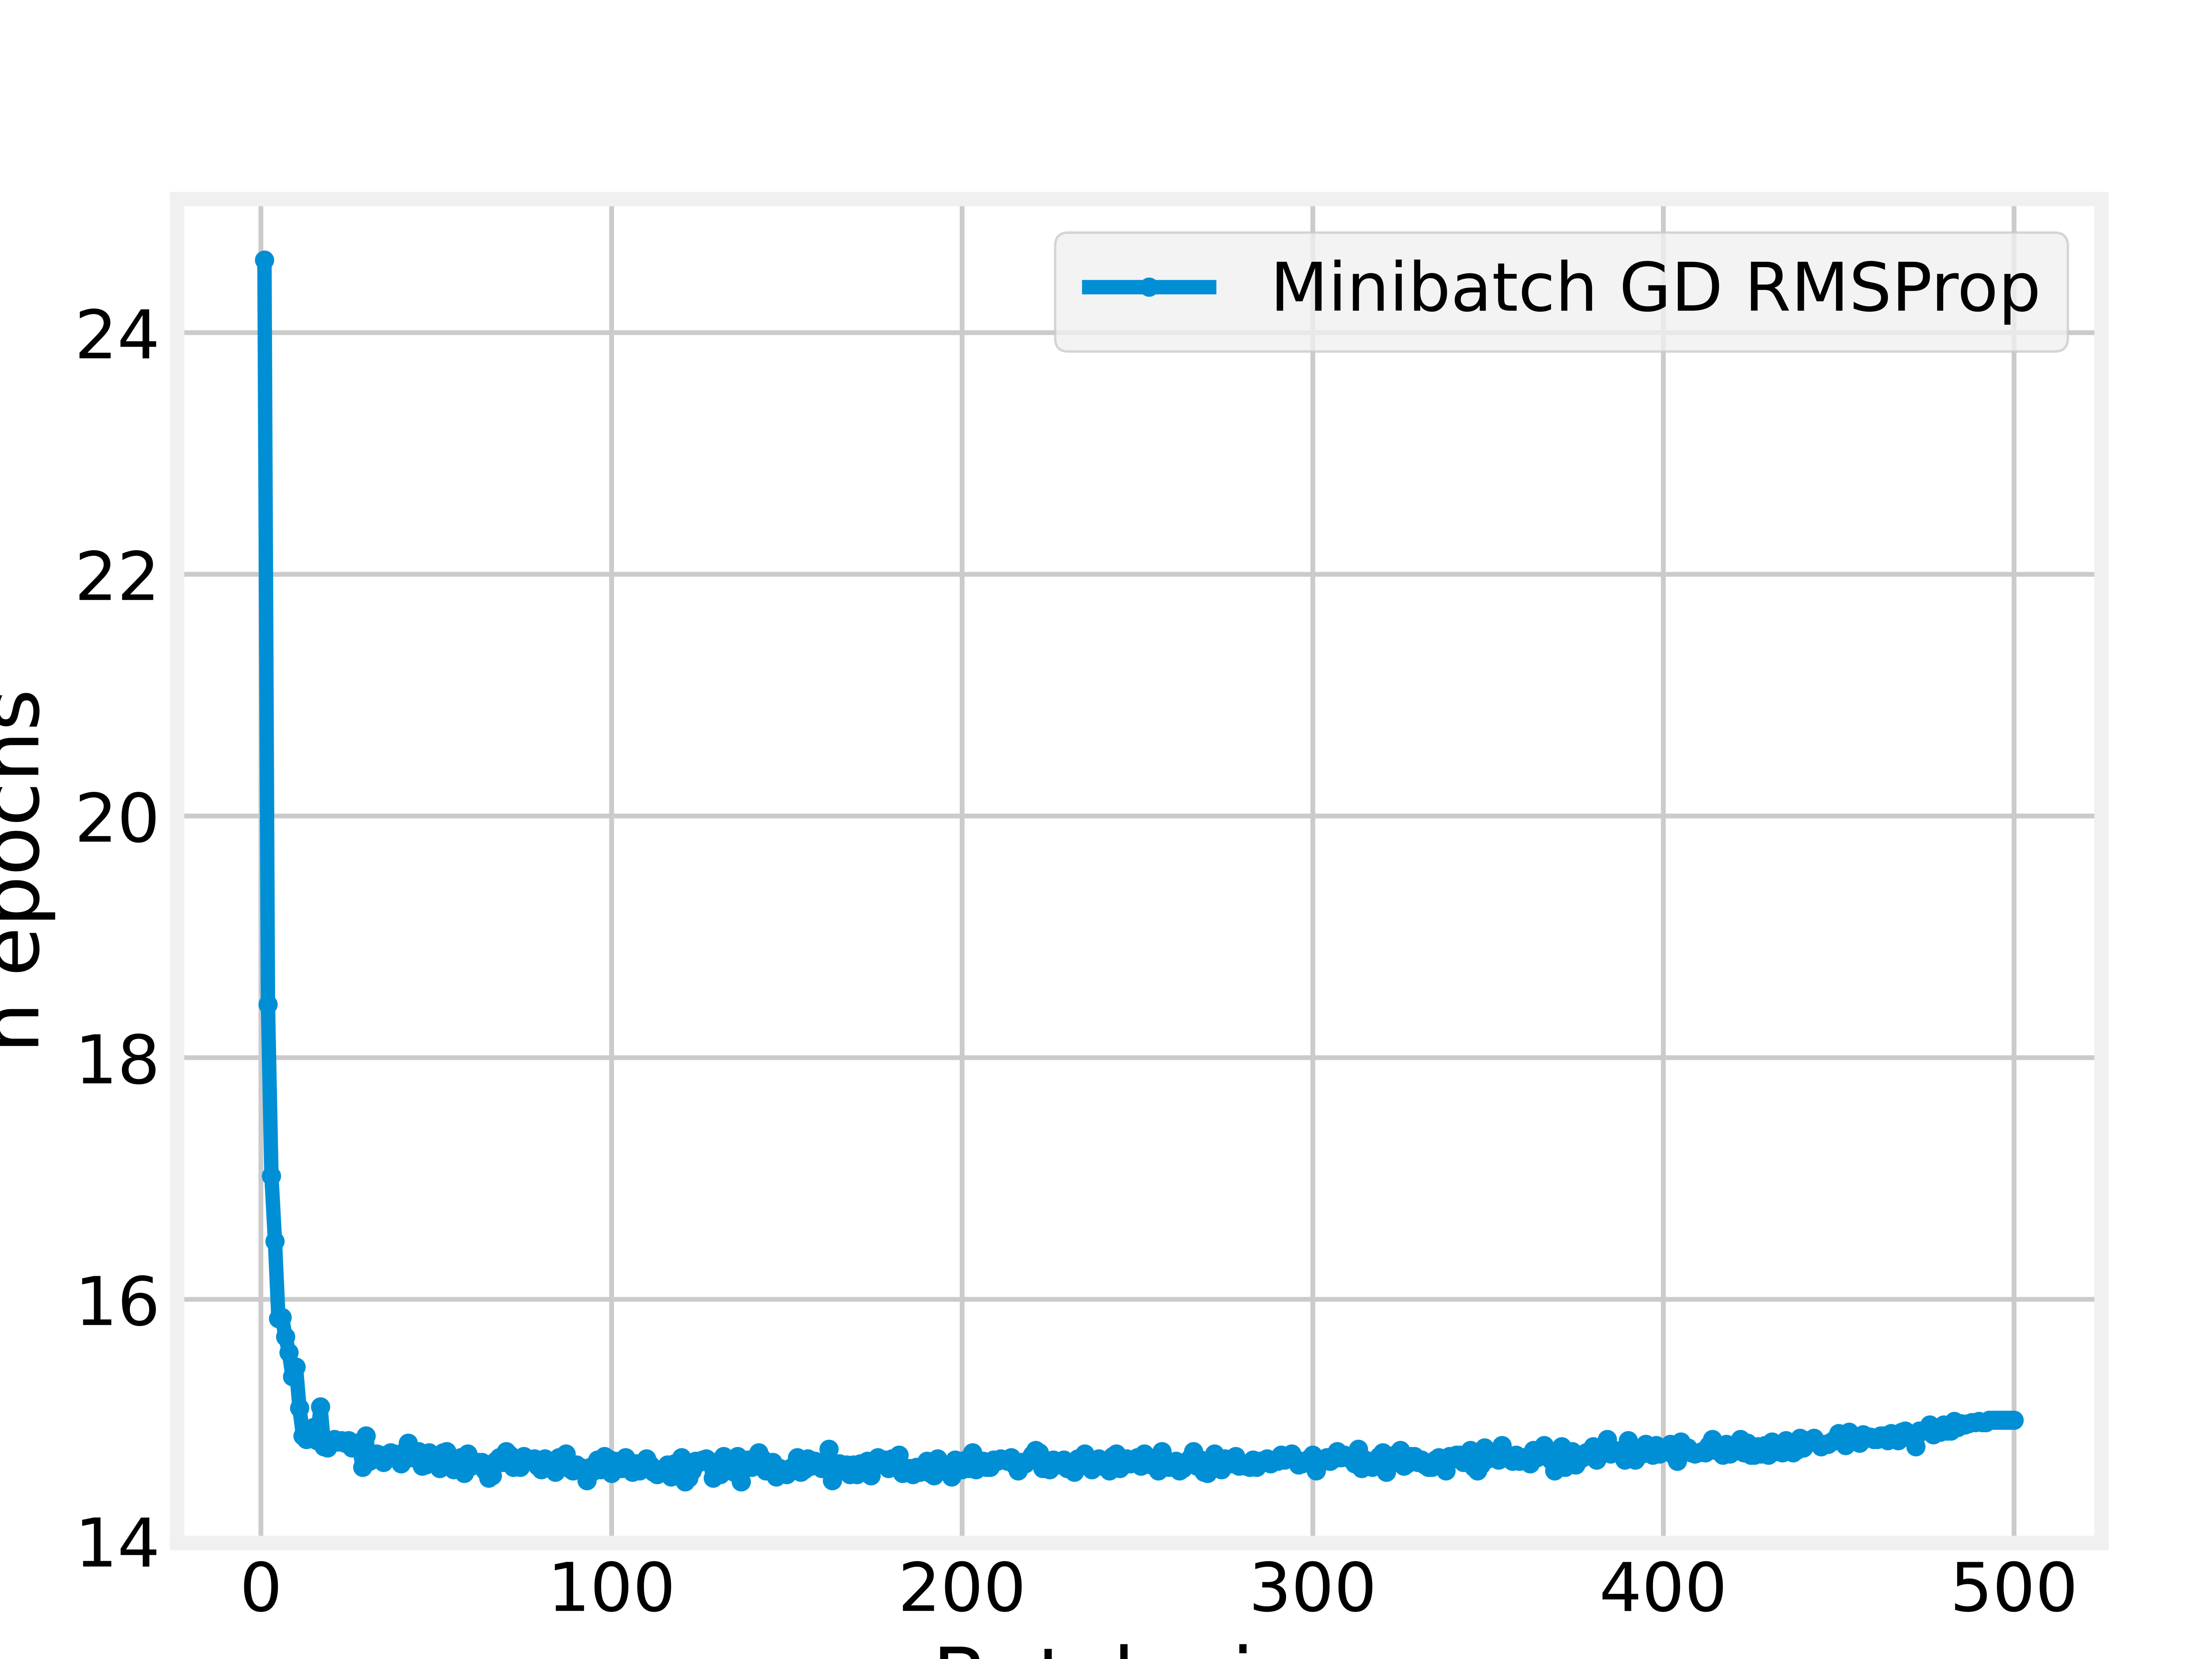
\includegraphics[scale = 0.9]{Image/T3_RMSPROP_GENERAL.png}
		\caption*{RMSProp in general}
	\end{figure}
	Даже анализа не нужно, чтобы понять, количество необходимых шагов до сходимости резко возрастает в связи с более равномерным изменением весов, одновременно решая глобальную проблему, тянувшейся еще с Momentum.

	Более детальное изображение RMSProp при первых десяти batch размерах:
	\begin{figure}[H]
		\centering
		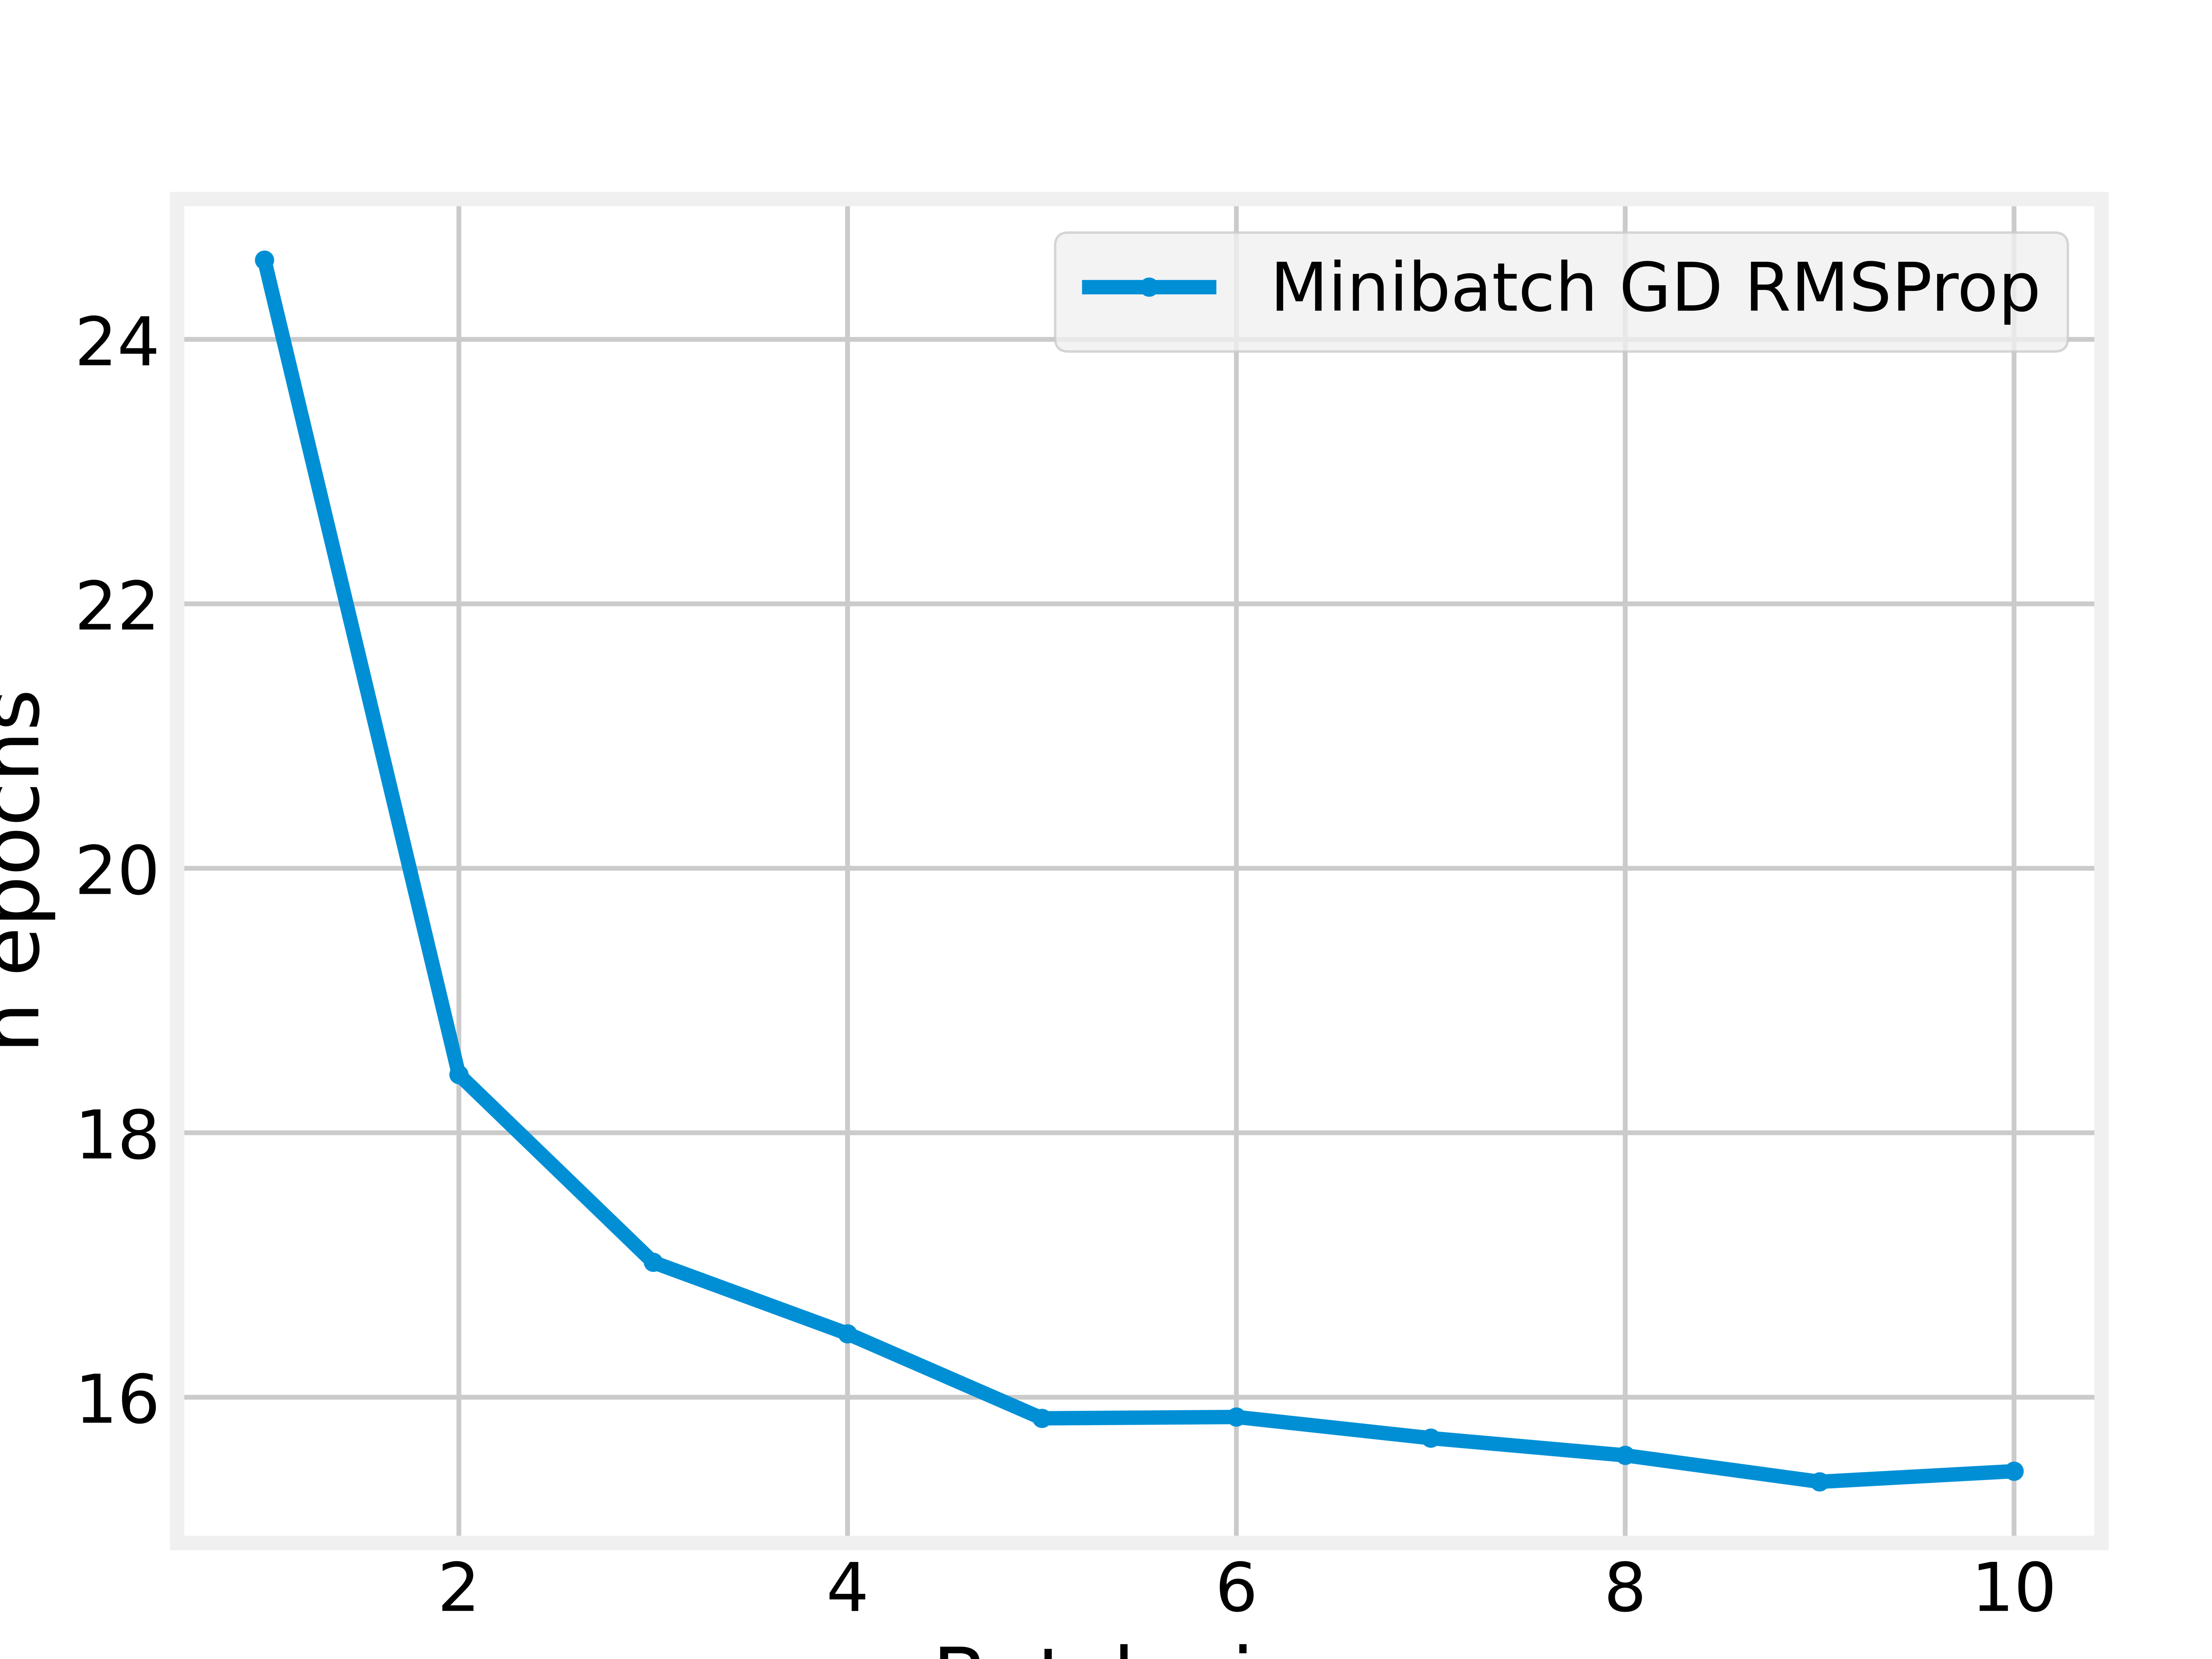
\includegraphics[scale = 0.9]{Image/T3_RMSPROP_1_10.png}
		\caption*{RMSProp in $[1, 10]$}
	\end{figure}
	\subsubsection*{Adam}
	Начинаем объединение веселья предыдущих.
	В отличие от всех его предшественником модификация \textit{Adam} является наиболее распространенным и используемым.
	\begin{align*}
		v_{i + 1} &= \lambda_{1} \cdot v_{i} + (1 - \lambda_{1}) \cdot g_{i} \\
		s_{i + 1} &= \lambda_{2} \cdot s_{i} + (1 - \lambda_{2}) \cdot (g_{i})^{2} \\
		\hat{v}_{i + 1} &= \dfrac{v_{i + 1}}{1 - \lambda_{1}^{i + 1}} \\
		\hat{s}_{i + 1} &= \dfrac{s_{i + 1}}{1 - \lambda_{2}^{i + 1}}
	\end{align*}
	Наконец, изменение весов будем рассчитывать по следующей формуле:
	\[
		w_{i + 1} = w_{i} - \lambda \cdot \dfrac{\hat{v}_{i + 1}}{\sqrt{\hat{s}_{i + 1} + \eth}},
	\] где $\lambda_{1} = 0.9$, $\lambda_{2} = 0.999$ и $\eth = 10^{-8}$.
	Настроим наше исследование и запустим с следующими параметрами:
	\begin{itemize}
		\item Максимальное количество эпох~-- $4000$.
		\item Начальным \texttt{learning\_rate}~-- $5e-1$.
		\item Количество генерируемых точек~-- $500$.
	\end{itemize}
	Рассмотрим же график для Adam.
	\begin{figure}[H]
		\centering
		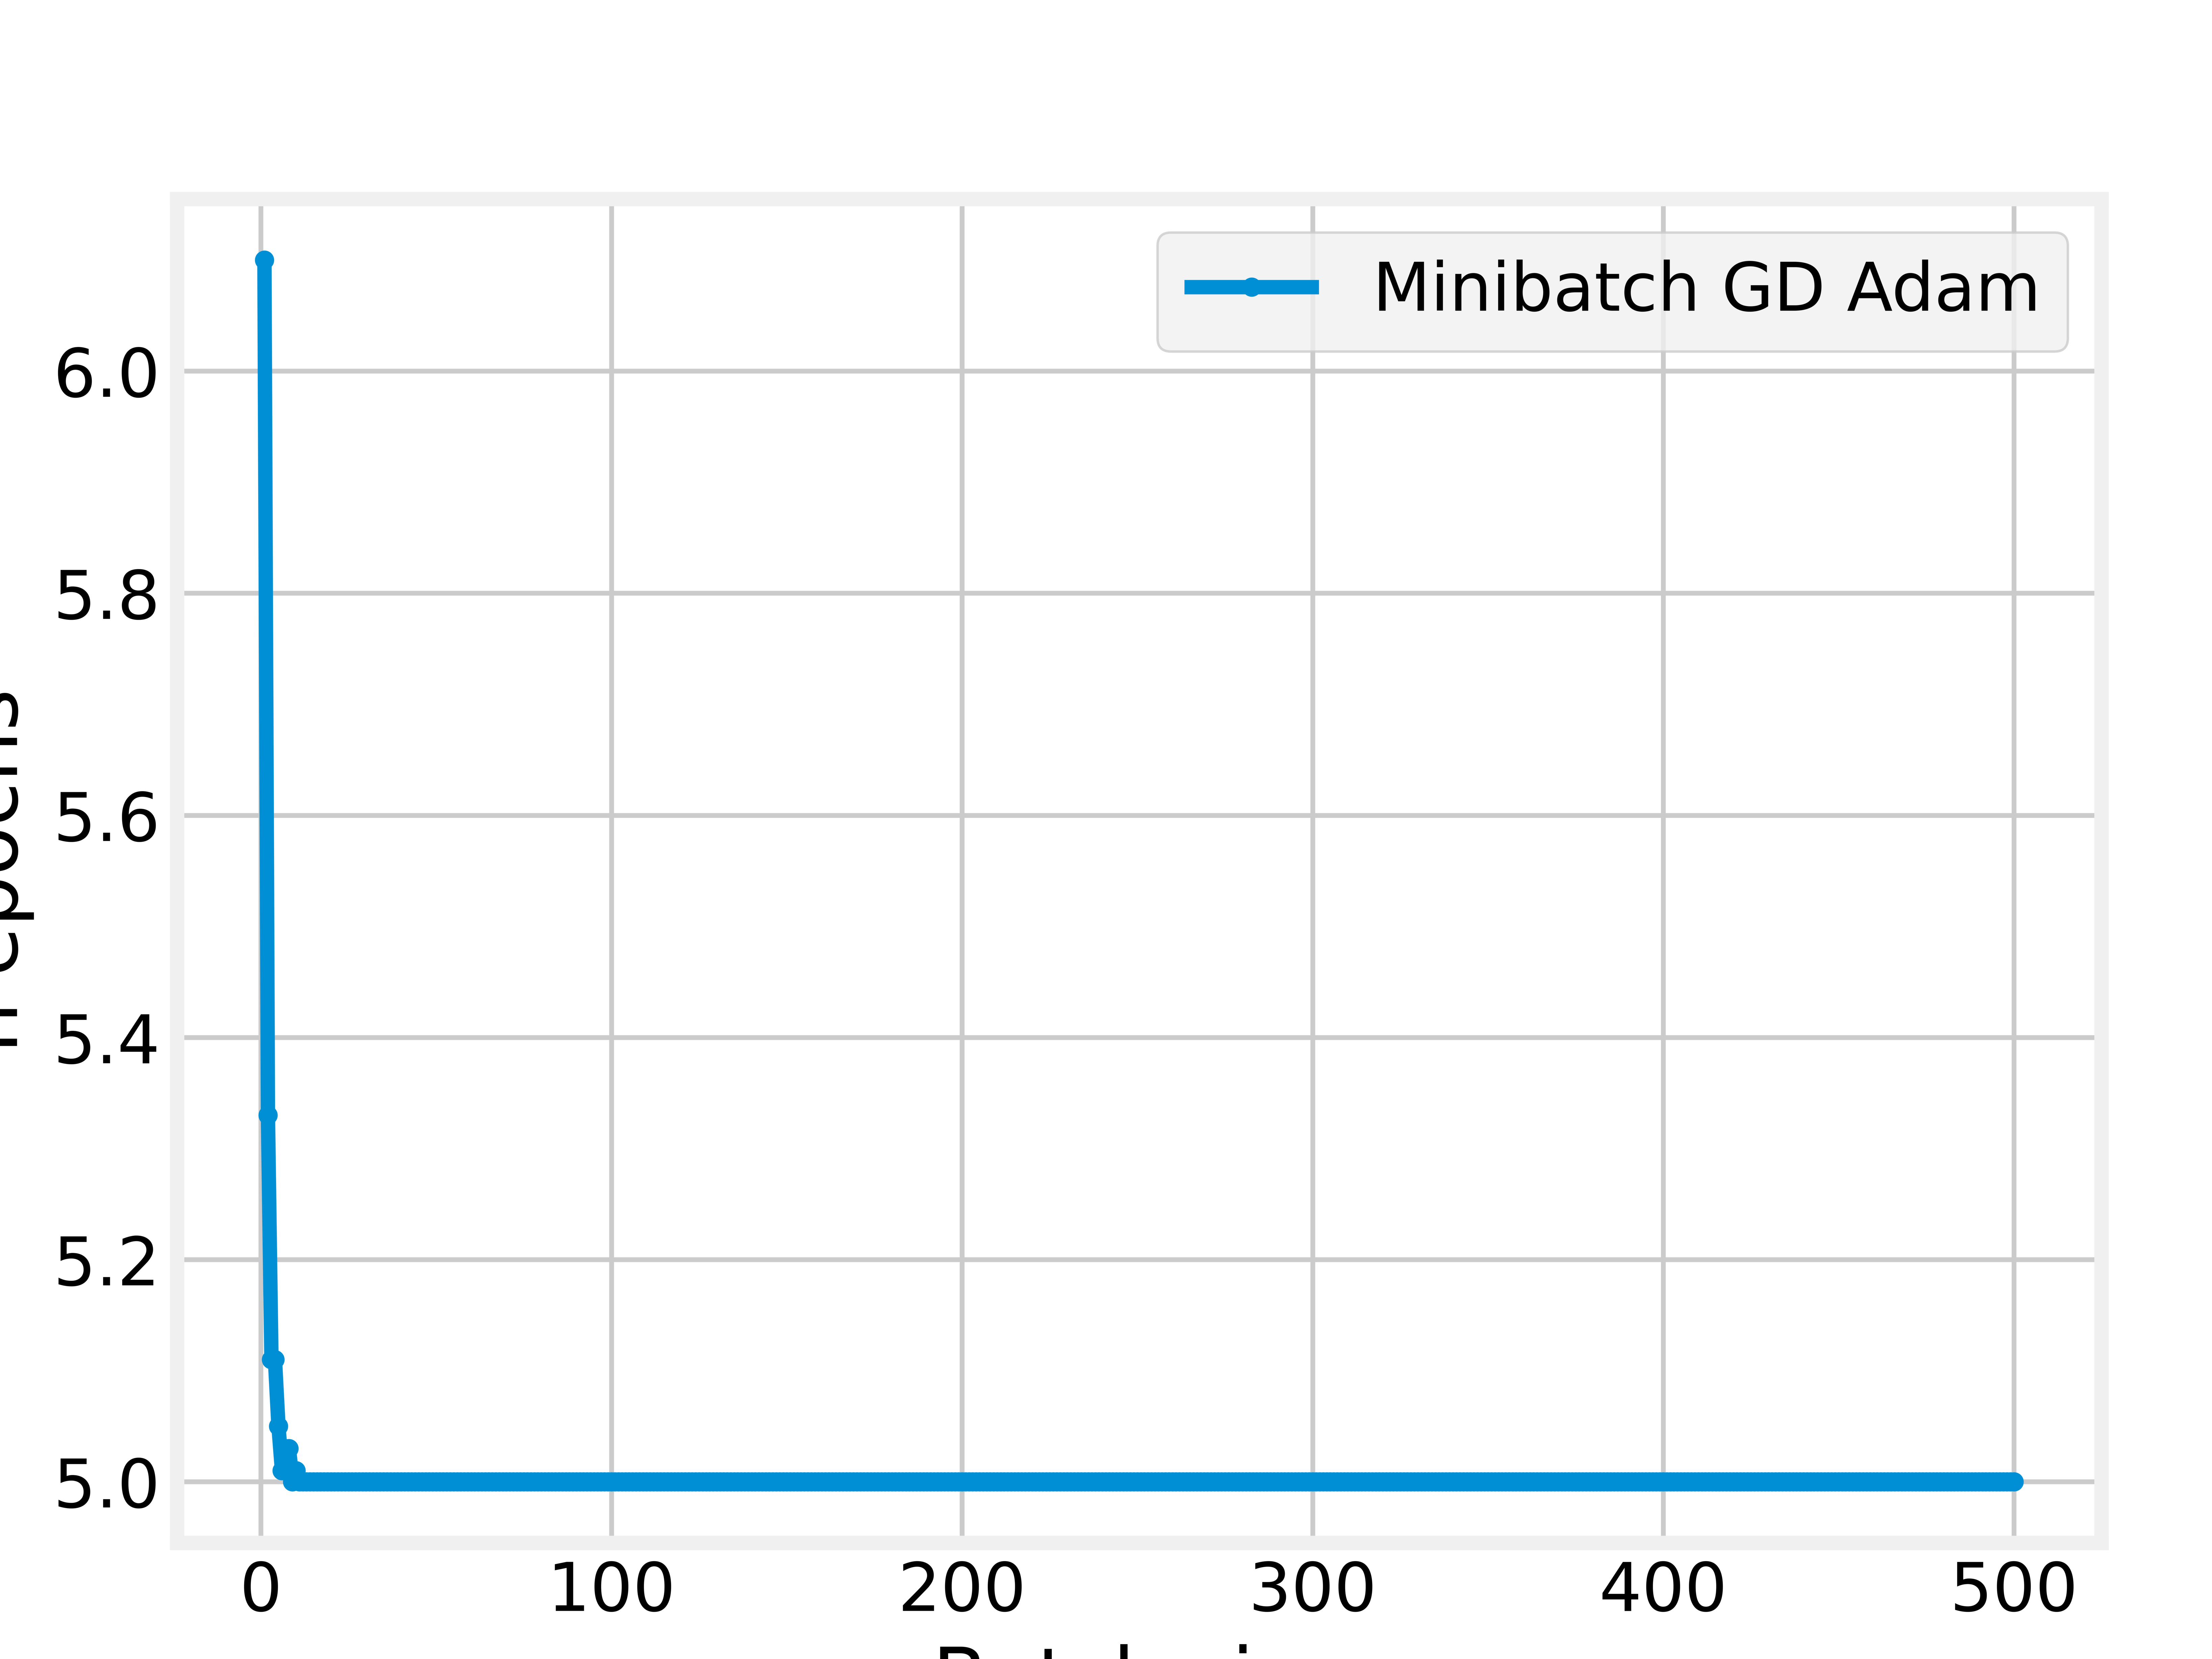
\includegraphics[scale = 0.9]{Image/T3_ADAM_GENERAL.png}
		\caption*{Adam in general}
	\end{figure}
	Даже анализа не нужно, чтобы понять, количество необходимых шагов до сходимости резко возрастает в связи с более равномерным изменением весов, одновременно решая глобальную проблему, тянувшейся еще с Momentum.

	Более детальное изображение Adam при первых десяти batch размерах:
	\begin{figure}[H]
		\centering
		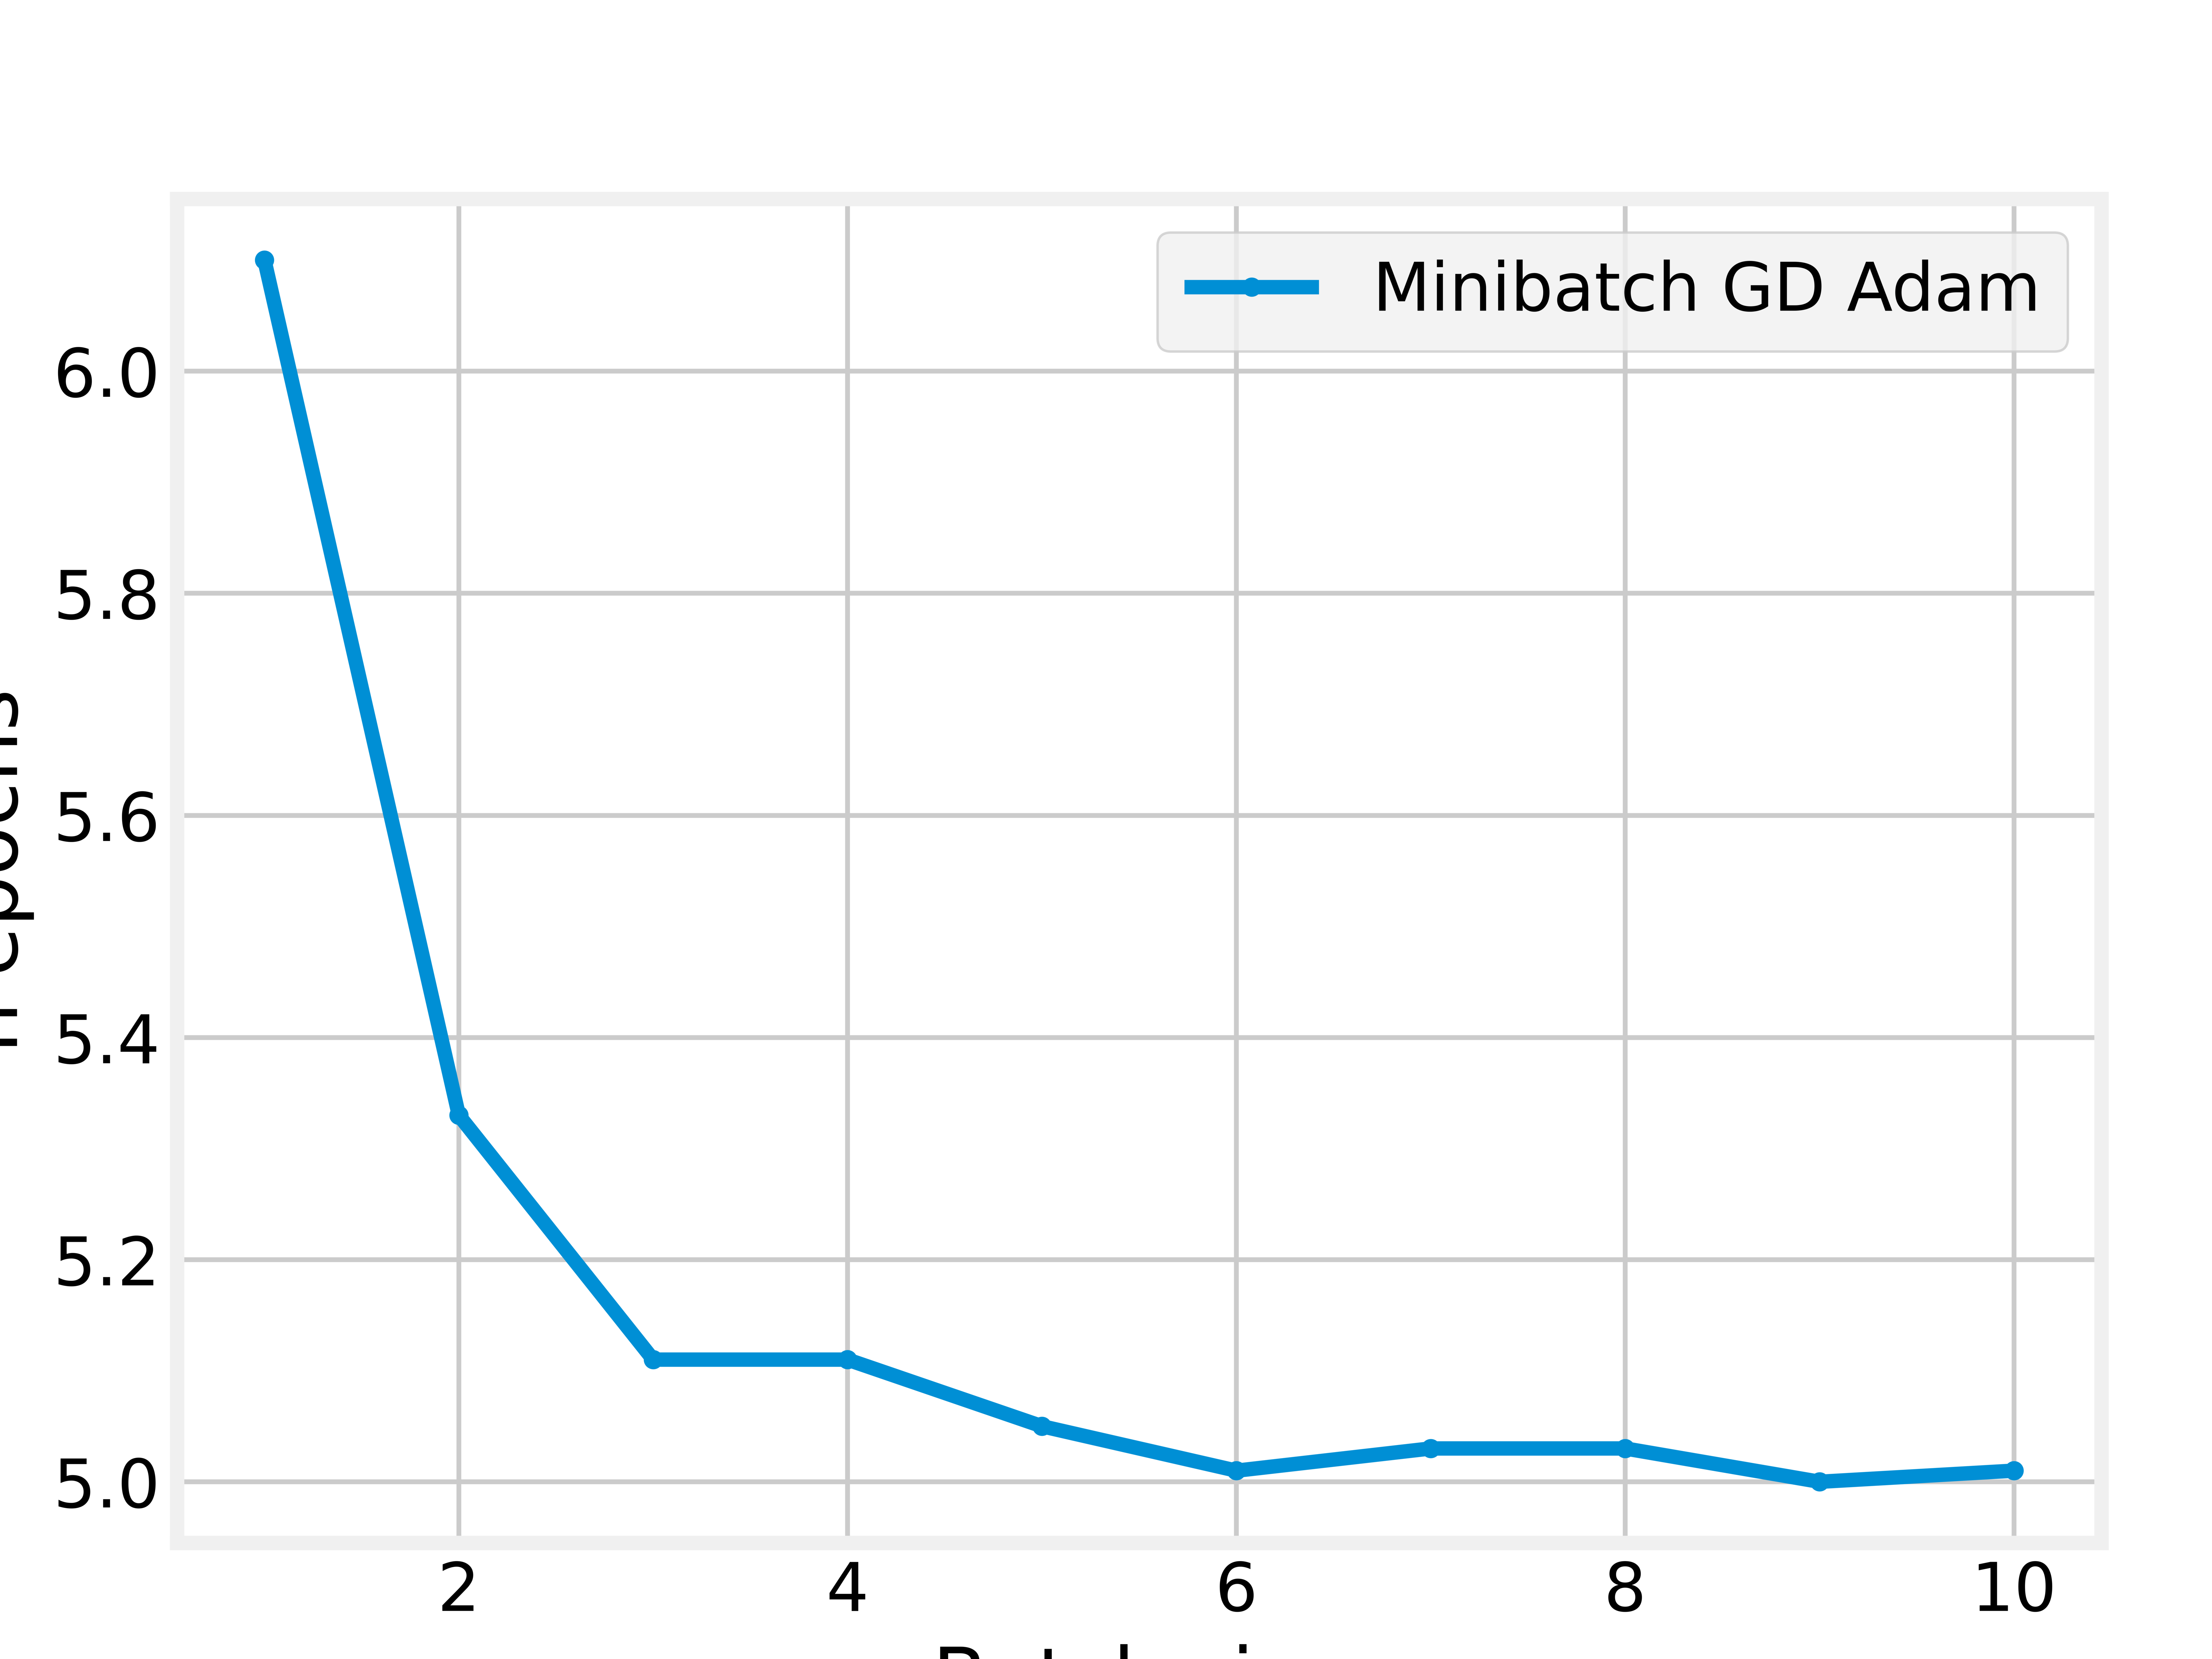
\includegraphics[scale = 0.9]{Image/T3_ADAM_1_10.png}
		\caption*{Adam in $[1, 10]$}
	\end{figure}
	\subsubsection*{Сравнение модификаций}
	\paragraph{Сходимость.}
	Ниже представлены графики зависимости времени и памяти на все созданные выше модификации с подписанными названиями.
	\begin{figure}[H]
		\centering
		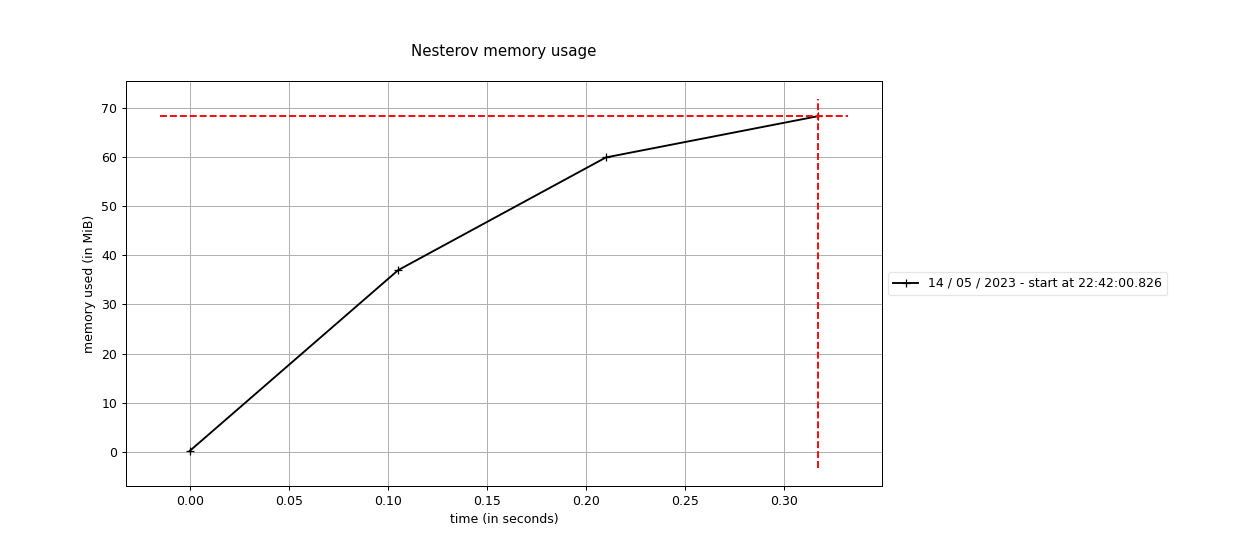
\includegraphics[scale = 0.6]{Image/T4_NESTEROV.png}
		\caption*{Nesterov/Time/Memory}
	\end{figure}
	\begin{figure}[H]
		\centering
		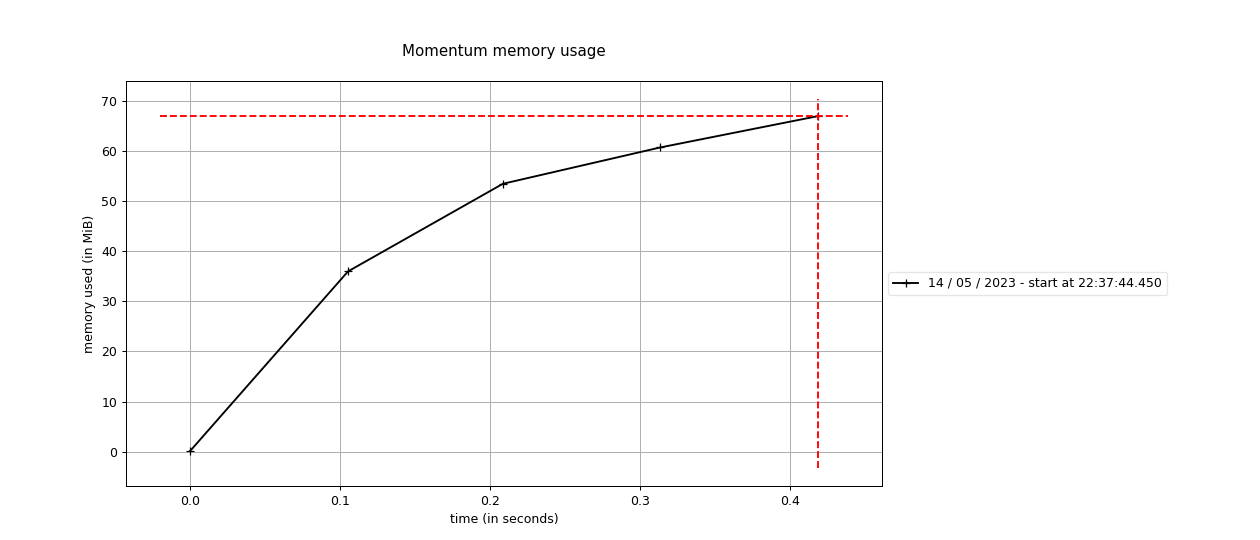
\includegraphics[scale = 0.6]{Image/T4_MOMENTUM.png}
		\caption*{Momentum/Time/Memory}
	\end{figure}
	\begin{figure}[H]
	\centering
	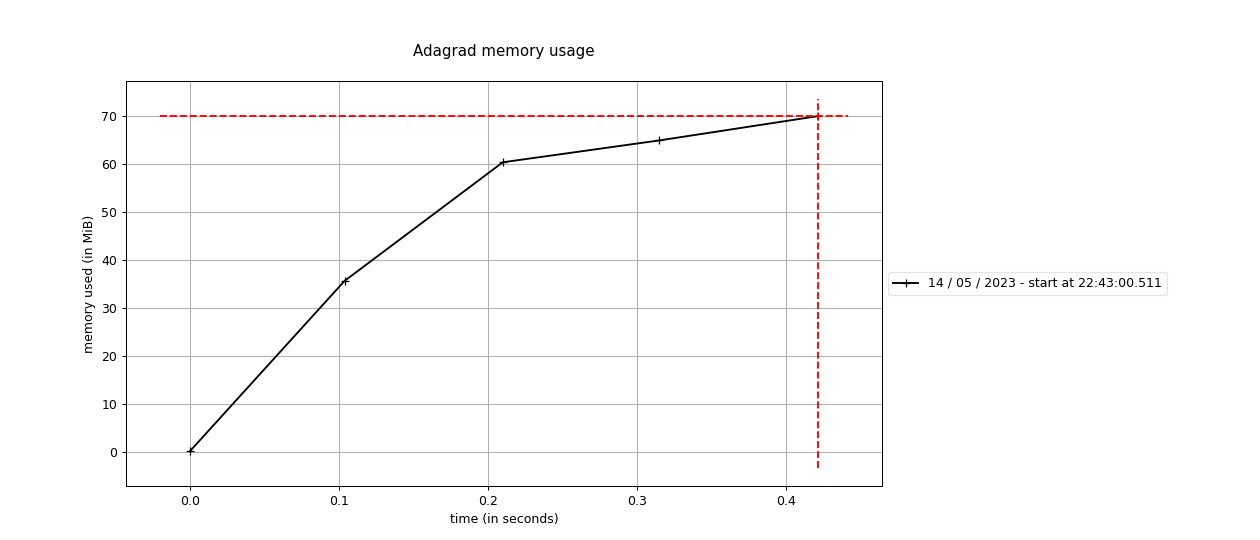
\includegraphics[scale = 0.6]{Image/T4_ADAGRAD.png}
	\caption*{AdaGrad/Time/Memory}
\end{figure}
	\begin{figure}[H]
	\centering
	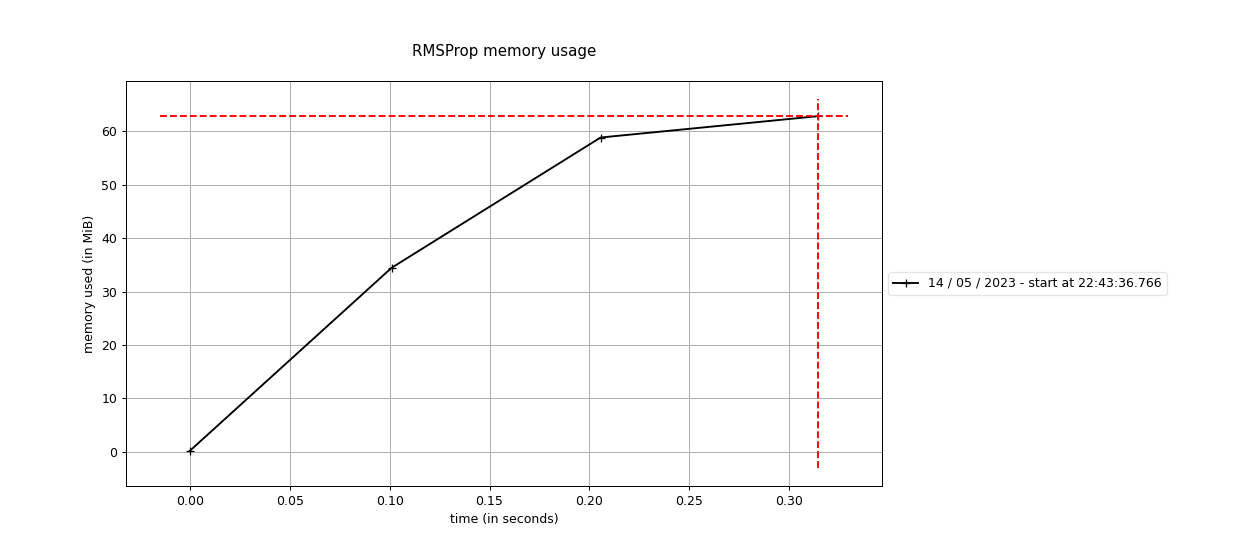
\includegraphics[scale = 0.6]{Image/T4_RMS.png}
	\caption*{RMSProp/Time/Memory}
\end{figure}
	\begin{figure}[H]
	\centering
	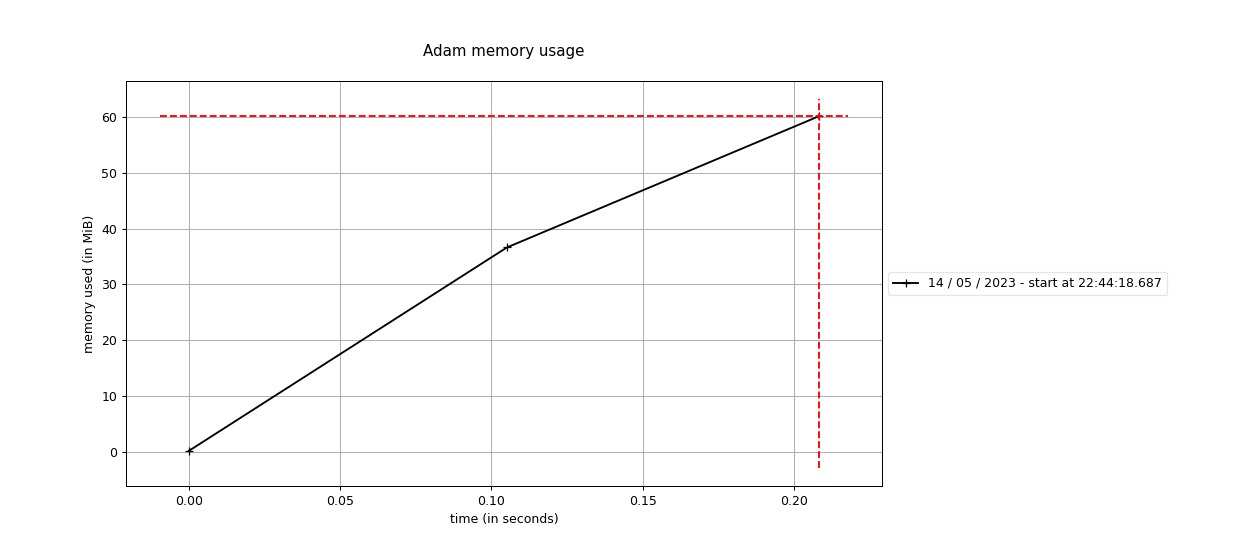
\includegraphics[scale = 0.6]{Image/T4_ADAM.png}
	\caption*{Adam/Time/Memory}
\end{figure}
	Также представим таблицу использования арифметических операций в разных функциях, которые имплементированы в модификациях.
		\begin{table}[H]
		\centering
		\begin{tabular}{|c|c|}
			Функция из имплементации & Количество арифметических операций \\ \hline
			\texttt{...\_with\_lr\_scheduling\_and\_moment} & 144539 \\
			\texttt{...\_with\_lr\_scheduling\_and\_nesterov\_moment} & 147550 \\
			\texttt{...\_with\_lr\_scheduling\_and\_adagrad} & 511881 \\
			\texttt{...\_with\_lr\_scheduling\_and\_RMSProp} & 48187 \\
			\texttt{...\_with\_lr\_scheduling\_and\_Adam} & 12055
		\end{tabular}
	\end{table}
	\paragraph{Траектории.}
	Траектория спуска различных алгоритмов из одной и той же исходной точки с одинаковой точностью.
	\begin{figure}[H]
		\centering
		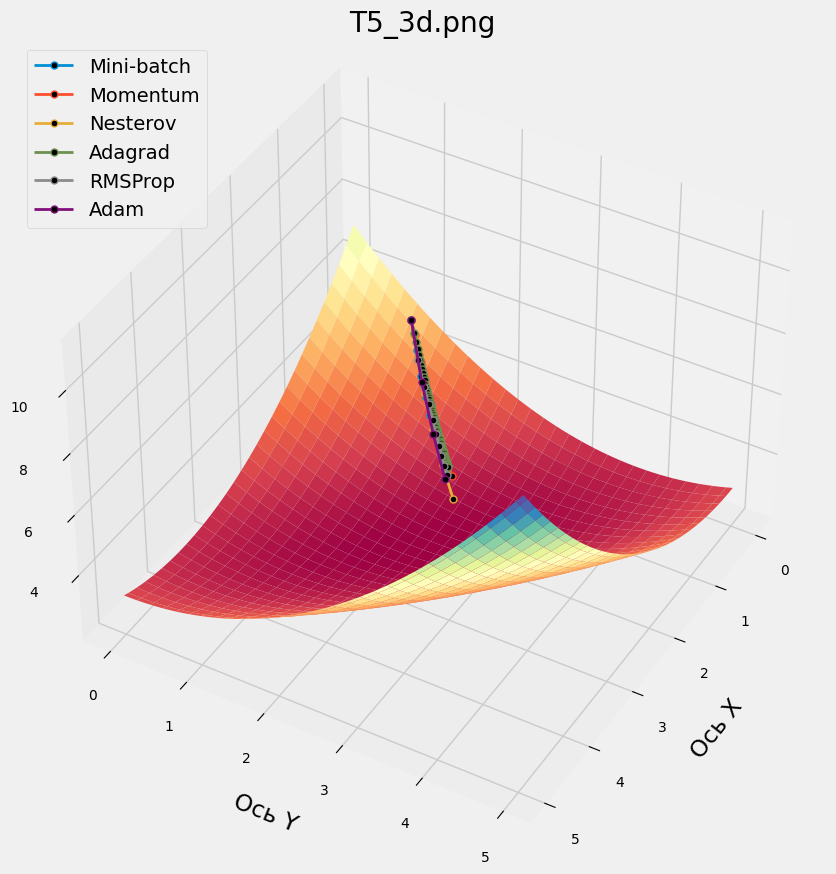
\includegraphics[scale = 0.6]{Image/T5_DIRECTIONS.png}
		\caption*{Directions}
	\end{figure}
	Рисунок с линиями равного уровня заданной функции.
	\begin{figure}[H]
		\centering
		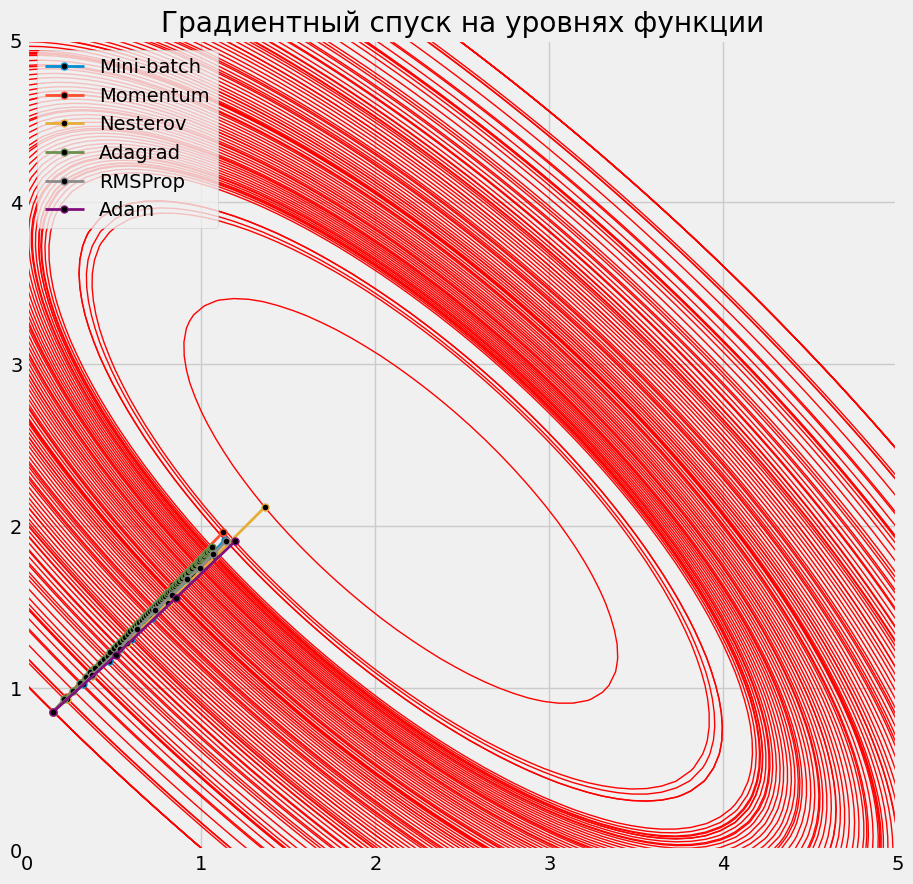
\includegraphics[scale = 0.6]{Image/T5_LINES.png}
		\caption*{Lines}
	\end{figure}
	\newpage
	\section*{Полиномиальная регрессия}
	\begin{enumerate}[1.]
		\item
		Реализуйте полиномиальную регрессию.
		Постройте графики восстановленной регрессии для полиномов разной степени.
		\item
		Модифицируйте полиномиальную регрессию добавлением регуляризации в модель (L1, L2, Elastic регуляризации).
		\item
		Исследуйте влияние регуляризации на восстановление регрессии.
	\end{enumerate}
	\subsection*{Введение}
	Представим себе некую функцию $f : \mathbb{R} \to \mathbb{R}$ причем такую, что она не зависит от каких-то побочных факторов (случайные значения и тому подобное), и при этом получаемые экспериментальные данные были как бы <<разбросаны>> относительно некой обобщающей кривой.
	Нашей задачей состоит в понимании, что это за кривая~-- по сути, это множество пар $M = \{\langle x, y\rangle : x \in \mathbb{R}, ~ y \in \mathrm{E}{(f(x))}\}$, которые при переходе от заданного $x' \to x''$ по некоторому $\delta$, подает предугадываемое значение $y''$ на основе полученных ранее начальных экспериментальных данных.
	Говоря простыми словами, с помощью данной прямой мы хотим получать прогноз.

	Рассмотрим идею \textit{полиномиальной регрессии}.
	Пусть даны $x_{i} \in X$ и $y_{i} \in Y$.
	Тогда уравнением полинома будет иметь следующий вид в нашей задаче:
	\[
		y_{i} = \sum\limits_{j = 0}^{k}{a_{j} \cdot x_{i}^{j}},
	\]
	где $\{a\}$~-- это коэффициенты полинома, где $a_{0}$, их мы ищем ровно тем же способом, что и в первой задаче~-- по методу наименьших квадратов.
	Наконец, по аналогии с задачей градиентного спуска, мы получаем следующее выражение:
	\[
		L = \omega \cdot \left\llbracket\sum\limits_{i = 1}^{n}{\left(\mathbf{y}_{i} - y_{i}\right)^{2}}\right\rrbracket \to \mathrm{min},
	\]
	где $\{\mathbf{y}\}$~-- это значения полинома в точках $\{x\}$, тогда наше выражение преобразуется:
	\[
		L = \omega \cdot \left\llbracket\sum\limits_{i = 1}^{n}{\left(\sum\limits_{j = 0}^{k}{\left(a_{j} \cdot x_{i}^{j} - y_{i}\right)^{2}}\right)^{2}}\right\rrbracket \to \mathrm{min},
	\]
	где $\omega = \dfrac{1}{n}$, для того чтобы усреднить квадратичные ошибки на всех обучающих примерах.
	Это позволяет получить более сбалансированную и интерпретируемую метрику ошибки, не зависящую от размера обучающей выборки.
	Для получения градиента исследуемой функции мы воспользуемся производной от $L$ по некоторому коэффициенту $a_{\mathbf{i}}$, тогда
	\[
		\dfrac{\partial{L}}{\partial{a_{\mathbf{i}}}} = 2 \cdot \omega \cdot \sum\limits_{i = 1}^{n}{\left(\sum\limits_{j = 0}^{k}{\left(a_{j} \cdot x_{i}^{j} - y_{i}\right) \cdot x^{i}_{\mathbf{i}}}\right)}
	\]
	\subsection*{Исследование различных модификация}
	Как и в задаче с градиентным спуском нам бы хотелось получать более реальные <<гладкие>> оценки предсказывания значения, вместо имения <<гор>> и <<впадин>> кривой.
	Эта проблема может быть решена с помощью модификаций к методу, которые, по своей сути, представляют из себя отдельные слагаемые.
	\subsubsection*{L1}
	Идея \textit{L1 регуляризации}.
	Давайте с каждой новой итерации мы будем неким способом <<наказывать>> нашу модель за высокие веса, чтобы в будущем увеличить обобщающую способность.
	Эта регуляризация основана на добавлении еще одного слагаемого в основную сумму, равного абсолютному значению коэффициентов полинома.
	\[
		L = \omega \cdot \sum\limits_{i = 1}^{n}{\left(\sum\limits_{j = 0}^{k}{\left(a_{j} \cdot x_{i}^{j} - y_{i}\right)^{2}}\right)^{2}} + \lambda \cdot \sum\limits_{i = 0}^{k}{\left(|a_{i}|\right)},
	\]
	где $\lambda$~-- есть общий коэффициент для регуляризации влияния штрафов на модель.
	Градиентом для модели будет выступать тогда такая формула:
	\[
		\dfrac{\partial{L}}{\partial{a_{\mathbf{i}}}} = 2 \cdot \omega \cdot \sum\limits_{i = 1}^{n}{\left(\sum\limits_{j = 0}^{k}{\left(a_{j} \cdot x_{i}^{j} - y_{i}\right) \cdot x^{i}_{\mathbf{i}}}\right)} + \lambda
	\]
	\subsubsection*{L2}
	Идея \textit{L2 регуляризации}.
	Данная модификация является небольшим дополнением к предыдущему в виде большей гладкости производной и возможностью лучшей работой с градиентным спуском.
	Проблема L1 заключалась в том, что в некоторых местах, где производная не может быть установлена, имеет резкие <<горы>>, <<впадины>> и вообще разрывы.
	Тогда, на помощью приходит немного иное штрафное значение функции~-- вместо суммы значений коэффициентов полинома мы возьмем квадраты.
	Отличает этот подход от L1 тем, что теперь мы штрафуем больше, но при этом никогда не зануляемся, как это было с предыдущей модификацией.
	\[
		L = \omega \cdot \sum\limits_{i = 1}^{n}{\left(\sum\limits_{j = 0}^{k}{\left(a_{j} \cdot x_{i}^{j} - y_{i}\right)^{2}}\right)^{2}} + \lambda \cdot \sum\limits_{i = 0}^{k}{\left(a_{i}^{2}\right)},
	\]
	где $\lambda$~-- есть общий коэффициент для регуляризации влияния штрафов на модель.
	Градиентом для модели будет выступать тогда такая формула:
	\[
		\dfrac{\partial{L}}{\partial{a_{\mathbf{i}}}} = 2 \cdot \omega \cdot \sum\limits_{i = 1}^{n}{\left(\sum\limits_{j = 0}^{k}{\left(a_{j} \cdot x_{i}^{j} - y_{i}\right) \cdot x^{i}_{\mathbf{i}}}\right)} + \lambda \cdot a_{\mathbf{i}}
	\]
	\subsubsection*{Elastic регуляризация}
	Идея \textit{Elastic регуляризация}.
	Объединение двух предыдущих идей, как и полезных особенностей, свойств обоих методов, при этом, корреляция переменных такая, что данная регуляризация не обнуляет некоторые из них, как в случае с L1.
	\[
		L = \omega \cdot \sum\limits_{i = 1}^{n}{\left(\sum\limits_{j = 0}^{k}{\left(a_{j} \cdot x_{i}^{j} - y_{i}\right)^{2}}\right)^{2}} + \lambda_{1} \cdot \sum\limits_{i = 0}^{k}{\left(a_{i}^{2}\right)} + \lambda_{2} \cdot \sum\limits_{i = 0}^{k}{\left(a_{i}^{2}\right)},
	\]
	где $\lambda_{1}$ и $\lambda_{2}$~-- есть коэффициенты для регуляризации влияния штрафов L1 и L2 на модель соответственно.
	Градиентом для модели будет выступать тогда такая формула:
	\[
		\dfrac{\partial{L}}{\partial{a_{\mathbf{i}}}} = 2 \cdot \omega \cdot \sum\limits_{i = 1}^{n}{\left(\sum\limits_{j = 0}^{k}{\left(a_{j} \cdot x_{i}^{j} - y_{i}\right) \cdot x^{i}_{\mathbf{i}}}\right)} + \lambda_{1} + \lambda_{2} \cdot a_{\mathbf{i}}
	\]
\end{document}
